\clearpage
\chapter{Event Selection, Signal and Control Regions}\label{sec:selections}

ROIs of all events inside the dataset listed in section ~\ref{sec:samples} are scored with the tensorflow, process trained with information from section ~\ref{sec:MLIV}.
Given that the signal process has 2 scalar decays as in Figure~\ref{fig:feynmanggH}, it's reasonable to require 2 high-scoring ROIs for our analysis.
(However, the 2 selected ROIs are not simply the 2 highest-scoring ROIs of the event, due to non-negligible lifetime of $\tau$ leptons (from signal process) in the detector.
%More detailed explanations are described in section~\ref{sec:lifetimeROI}.)  
The cuts on the leading ROI, and the subleading ROI are optimized based on maximizing the punzi significance formula with value $\sigma$ set to discovery value of 5.  
\begin{equation}\label{eq:significance}
    \sigma(N_{\mathrm{displaced-tag}}) = \frac{S(N_{\mathrm{displaced-tag}})} {\sqrt{B(N_{\mathrm{displaced-tag}})} + 2.5 }.
\end{equation}


 \begin{figure}[h!]
   \caption{Signal versus Background for log10(1-ROIscore), where the ROI score is the highest ROI of the event. Left plot is for MS-15\_ctauS-10mm point, whereas the right plot is for MS-15\_cauS-100mm point}
   \label{fig:leadROIscore}
   \centering
   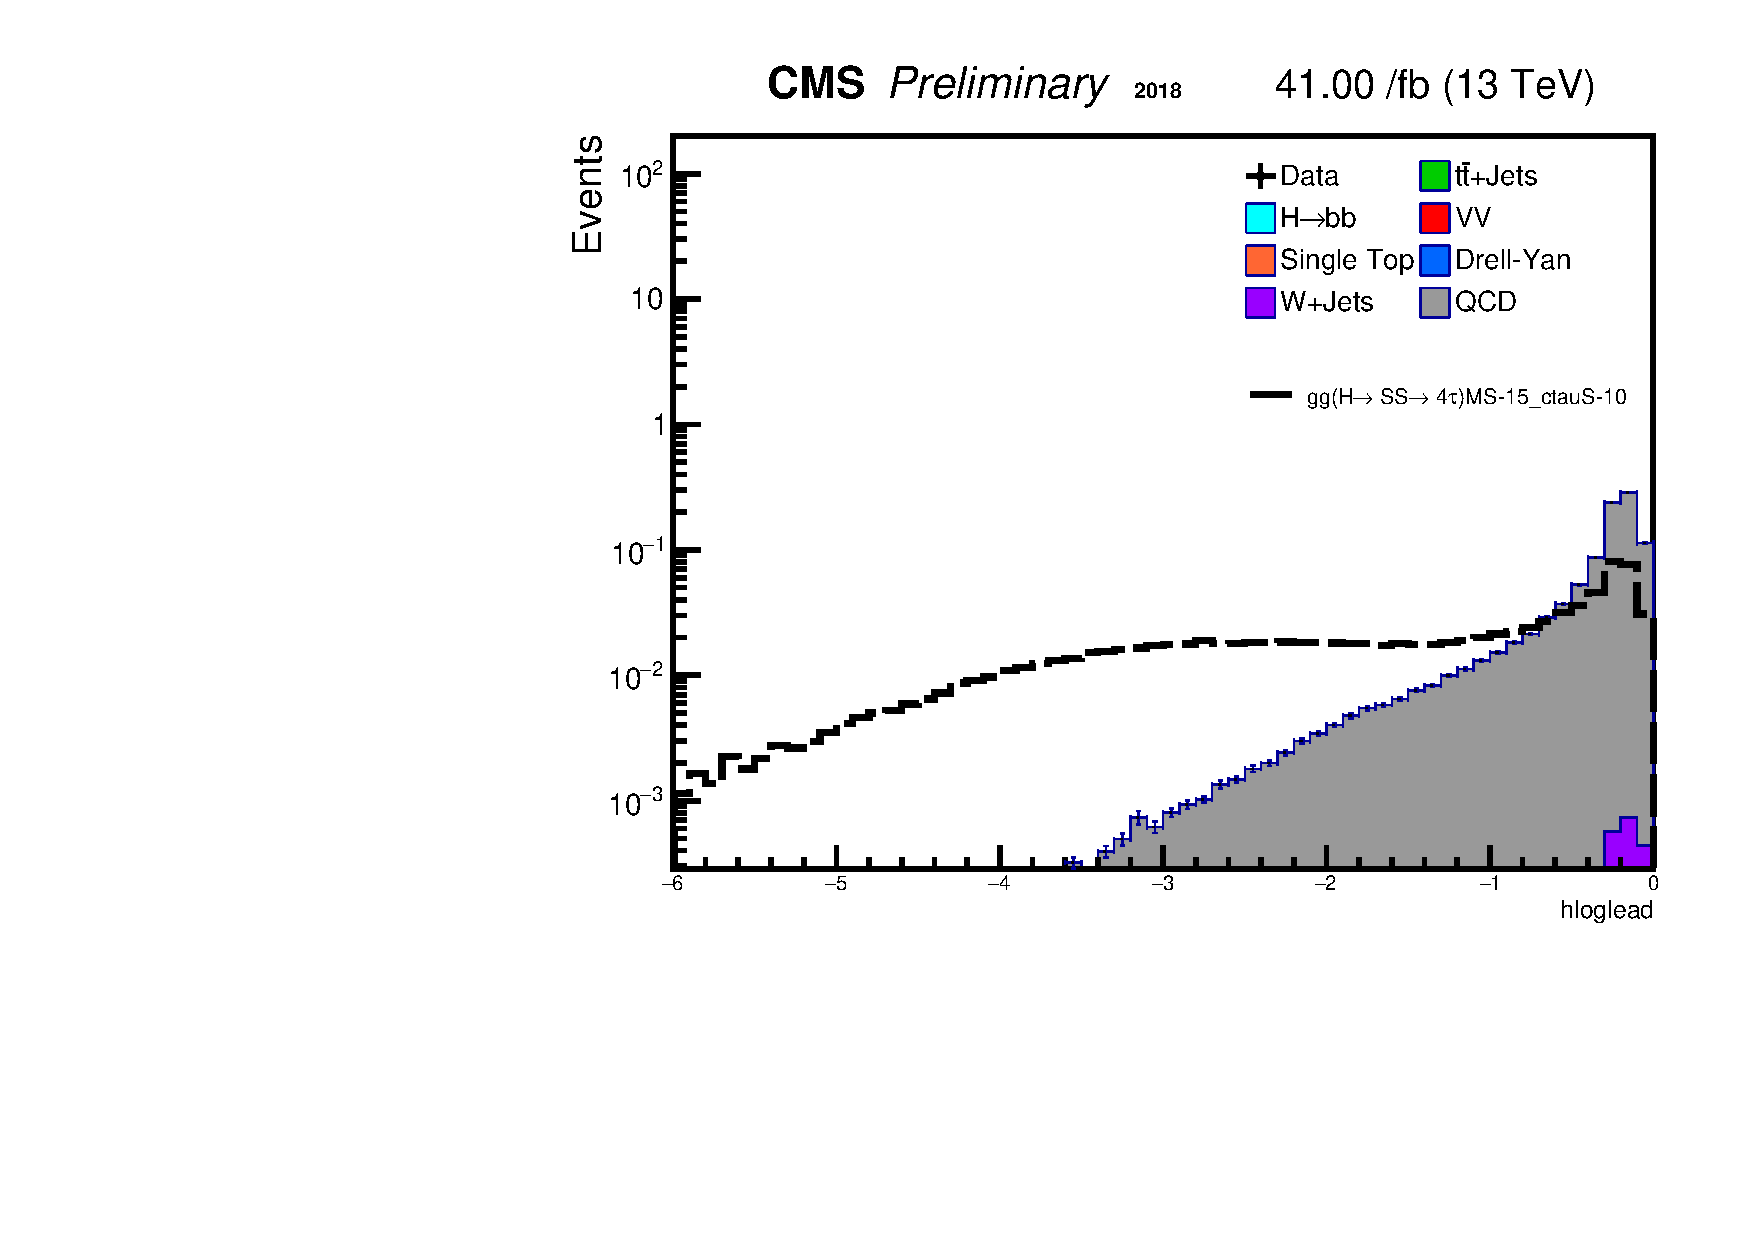
\includegraphics[width=0.47\linewidth]{figs/AnalysisNoteplot_MS-15_ctauS-10_hloglead.pdf}
   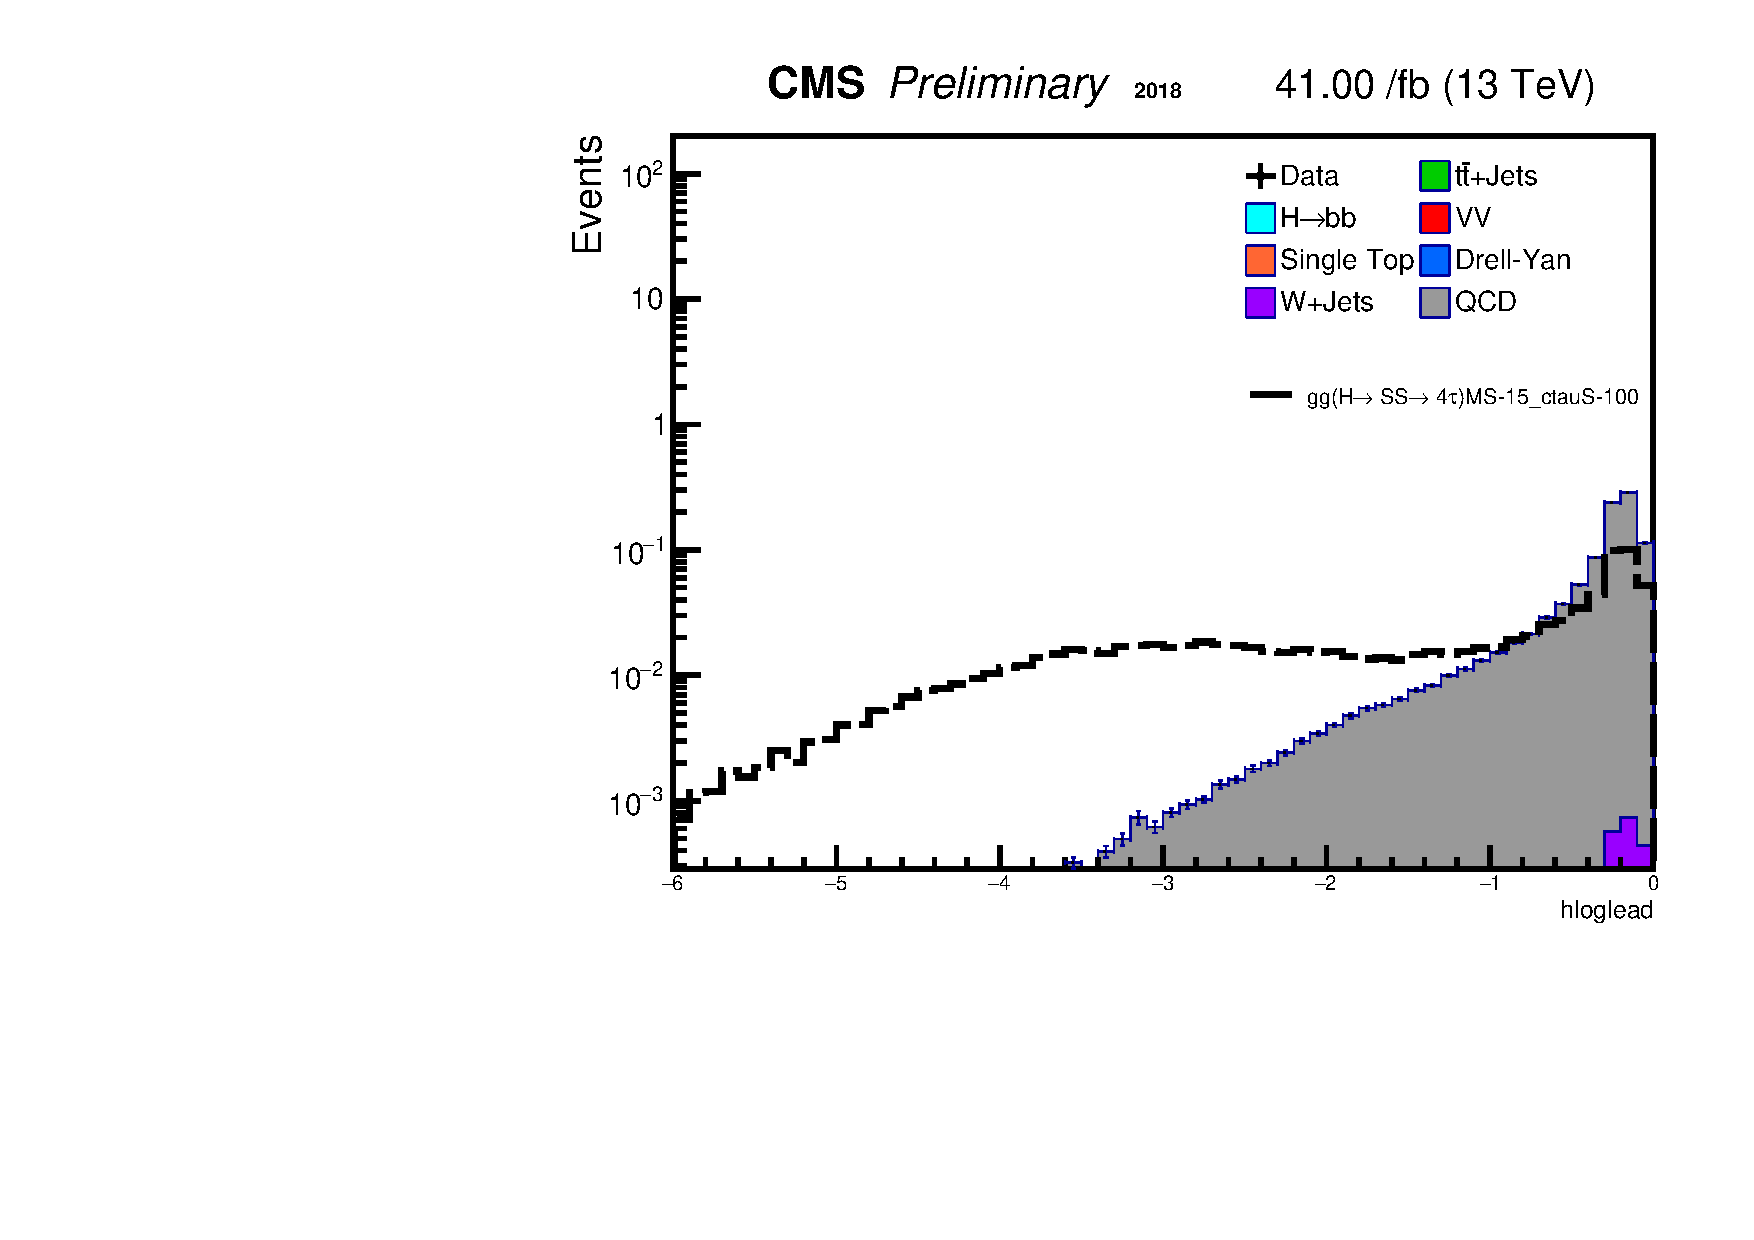
\includegraphics[width=0.47\linewidth]{figs/AnalysisNoteplot_MS-15_ctauS-100_hloglead.pdf}
 \end{figure}


 \begin{figure}[h!]
   \caption{Signal versus Background for log10(1-subROIscore), where the ROI score is the second highest ROI (outside of dPhi=0.4 from leading ROI) of the event. Left plot is for MS-15\_ctauS-10mm point, whereas the right plot is for MS-15\_cauS-100mm point}
   \label{fig:excROIscore}
   \centering
   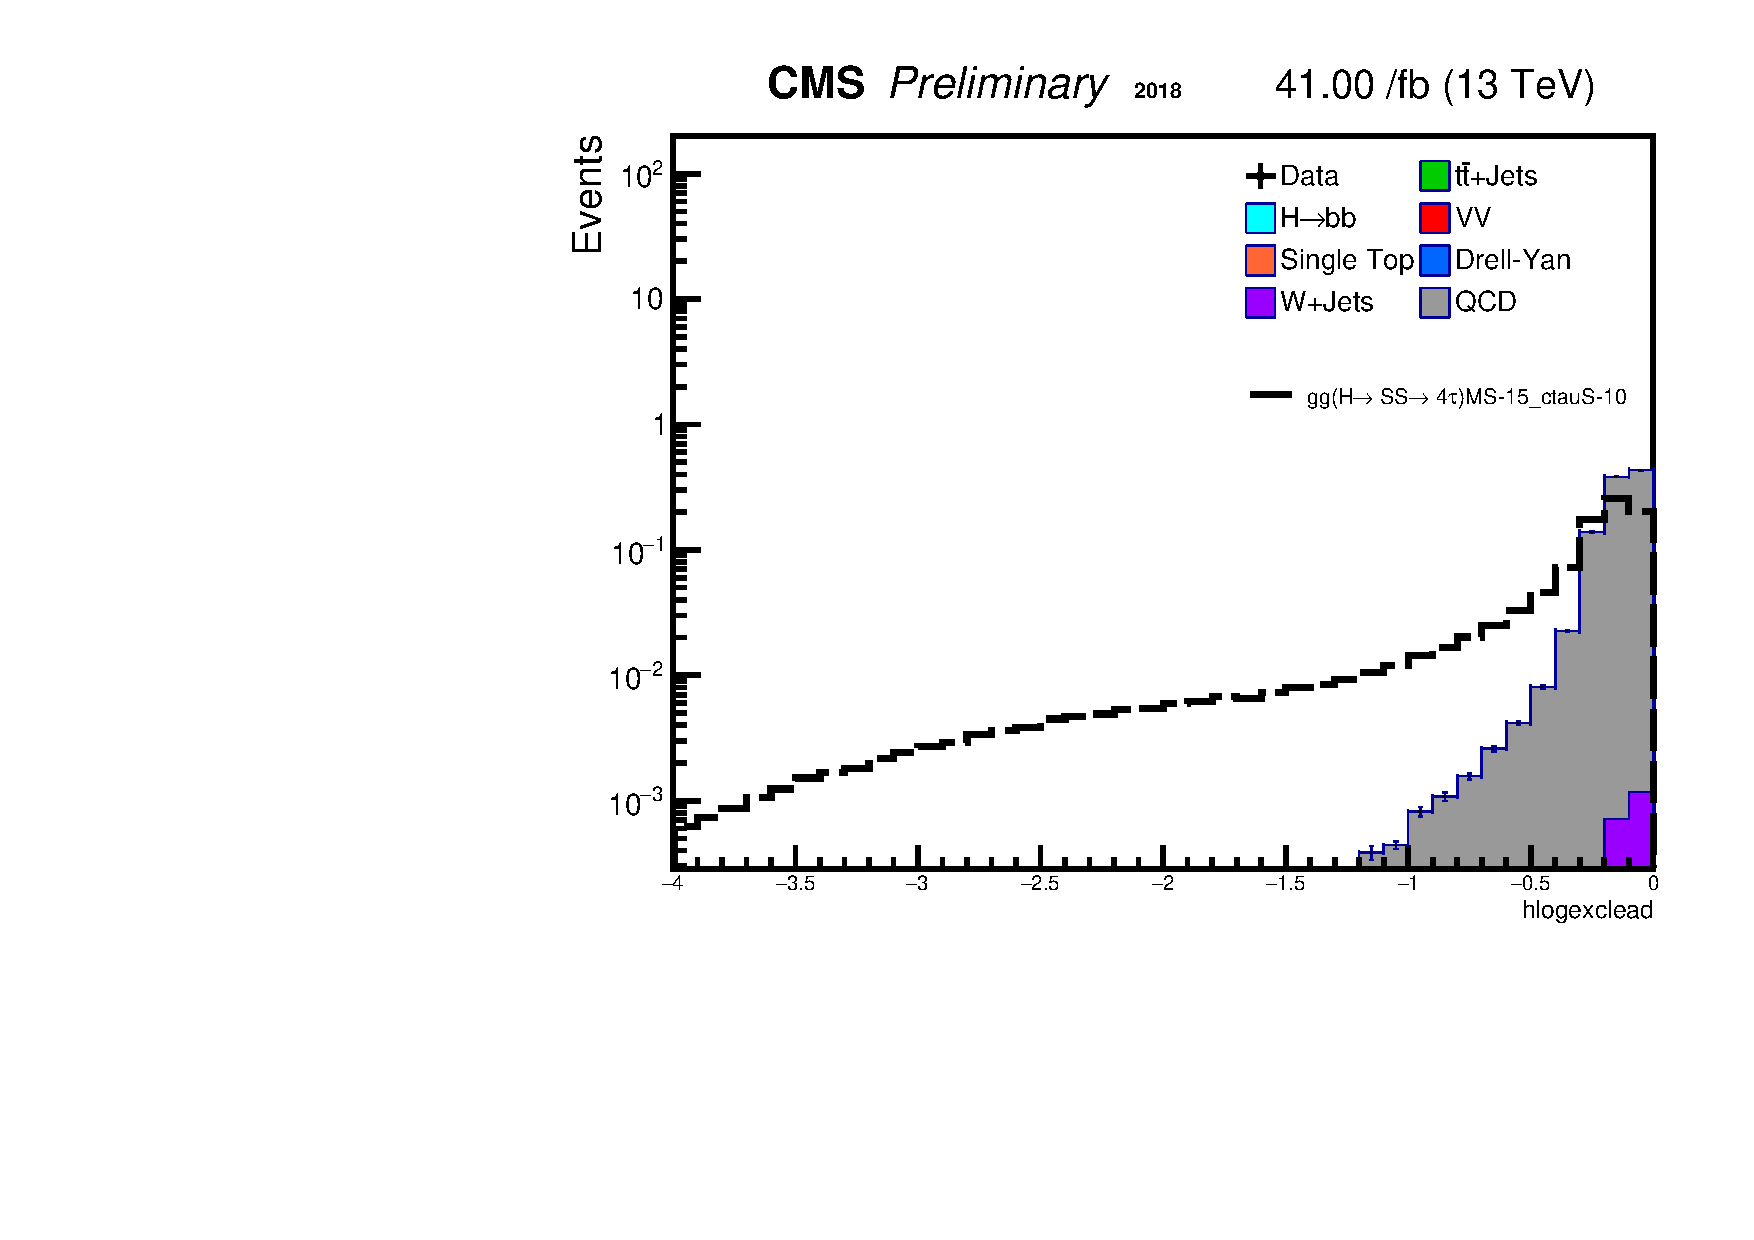
\includegraphics[width=0.47\linewidth]{figs/AnalysisNoteplot_MS-15_ctauS-10_hlogexclead.pdf}
   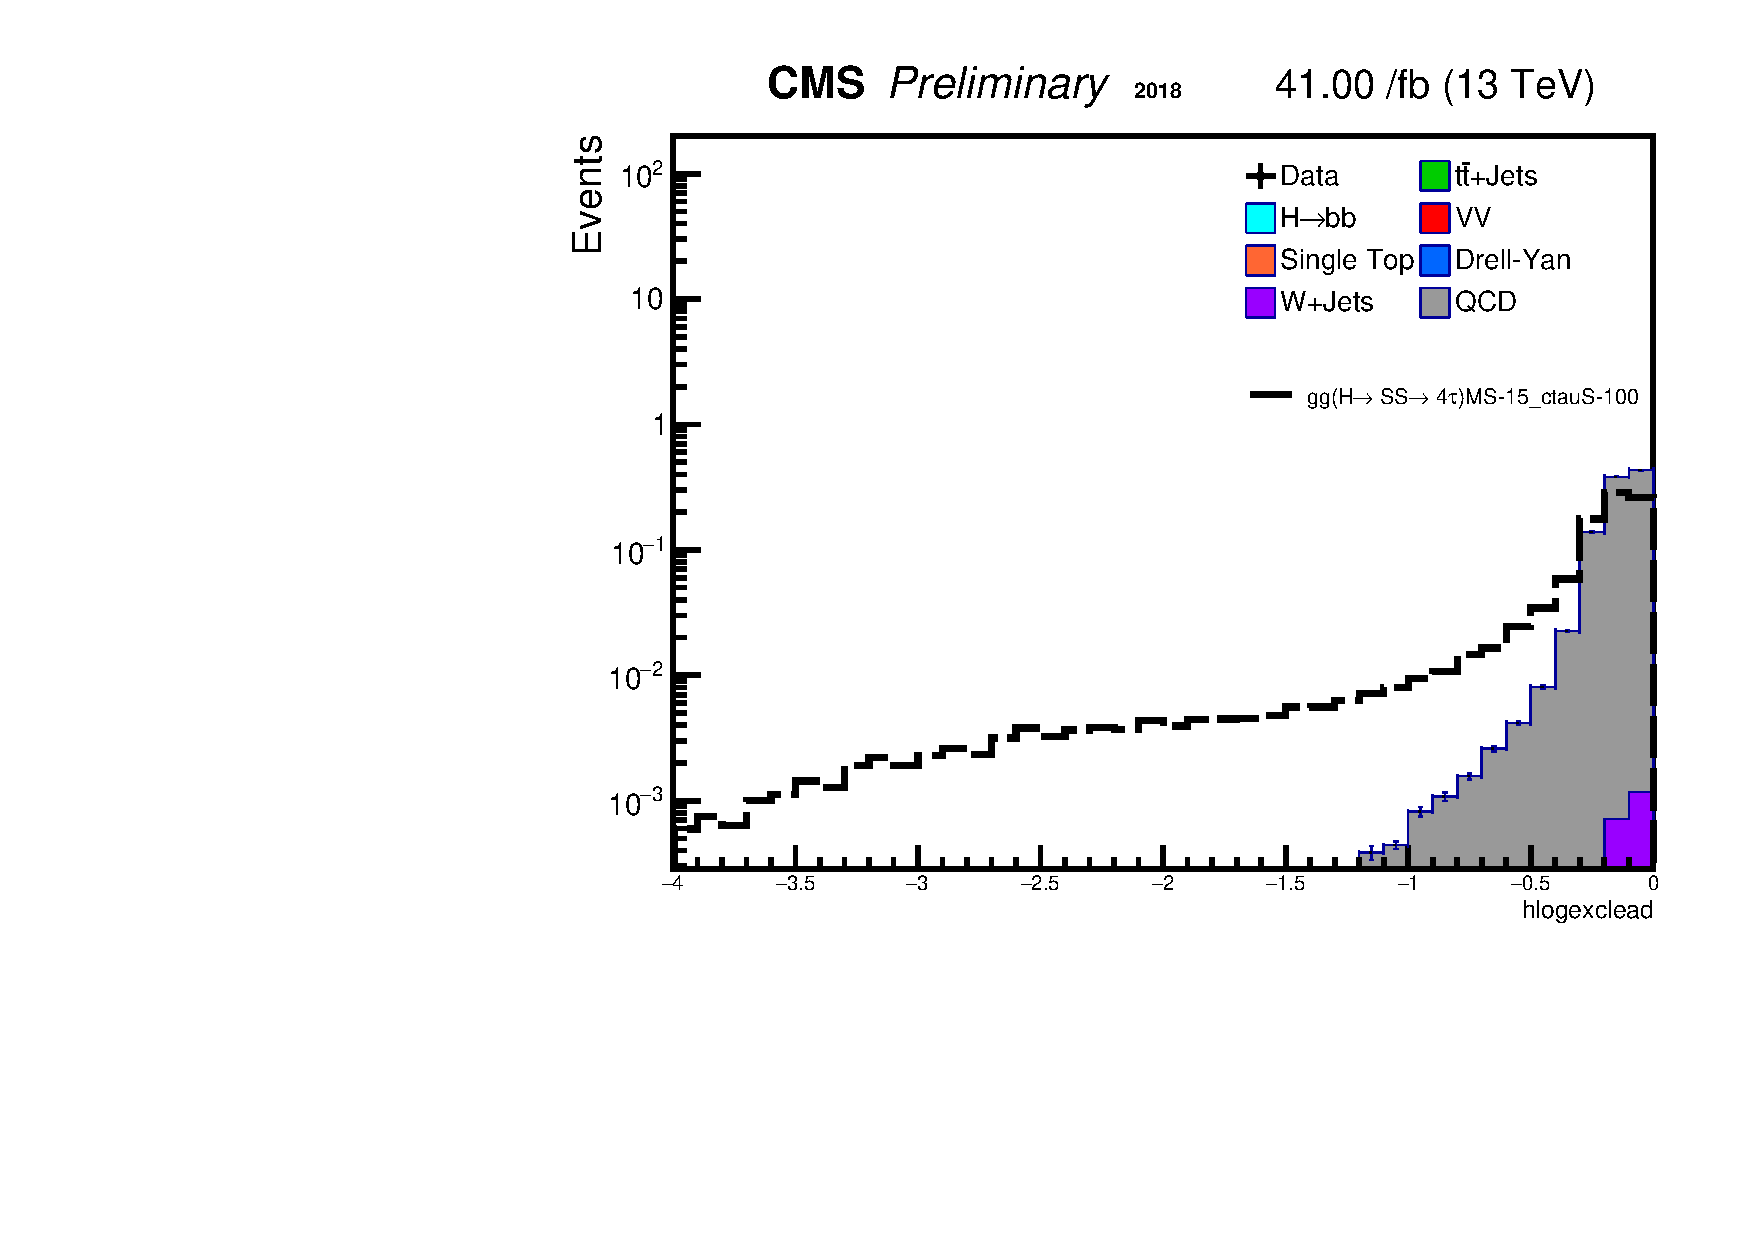
\includegraphics[width=0.47\linewidth]{figs/AnalysisNoteplot_MS-15_ctauS-100_hlogexclead.pdf}
 \end{figure}

%% \begin{figure}[h!]
%%   \caption{Trigger turn-on curves for the 17 MuonEG HLT path. Leading \pt
%%   lepton (left) and subleading \pt lepton (right).}
%%   \label{fig:17_trigger_turnon_mueg}
%%   \centering
%%   \includegraphics[width=0.40\linewidth]{figs/2017_TTOCEMu_ElePt.png}
%%   \includegraphics[width=0.40\linewidth]{figs/2017_TTOCEMu_MuPt.png}
%% \end{figure}

In addition, we have other cuts applied throughout the analysis.
These variables are either
\begin{itemize}
 \item Non-relevant to ROIs (muon, jet object)
 \item Construction of geometric variable after selecting 2 highest scoring ROIs.
 \item Missing input variable in ROI training
\end{itemize}
These are not inputs of ML training, something that can't be learned by the ML, so not discriminated with scoring of the ROIs.

They include 
\begin{itemize}
  \item $\Delta\Phi(lead ROI,sublead ROI)$ 
  \item Number of Annulus tracks associated with ROI $<$ 8
  \item 1 Isolated $\mu$
  \item $\Delta R(lead ROI, Jet)<$0.6 
  \item Leading $\mu$'s transverse impact parameter to PV $>$ 0.1
\end{itemize}

Each of the cuts for the items above is motivated and explained in following subsections.

\section{Delta Phi(lead ROI,sublead ROI)}\label{sec:DeltaPhi}
This analysis looks for displaced vertices in the tracker region, coming from the decays of exotic LLPs from Higgs produced in gluon fusion mode, leaving the SM Higgs boson without boost.
The largest mass of the exotic LLPs is 55 GeV, ranging down to 7 GeV. 
Thus, exotic LLPs decayed from the SM Higgs become boosted, with their momentum vectors pointing back-to-back in the SM Higgs rest frame. 
Exotic LLPs with lighter mass are more boosted than heavier LLPs, since less LLP mass means more leftover energy into kinetic energy.
Given that ROIs corresponding to an exotic LLP's decay should have the highest ROI score, one should expect that the leading ROI and subleading ROI in a single event would be back-to-back.
Thus, in signal events, $\Delta\Phi$(lead ROI,sublead ROI) tends to have high values, while the background processes tend to have a more uniform distribution.
This analysis applies a cut above 2.2 to reduce background contribution. 
Optimization process for this variable is detailed in here (To be done in future?)
%Figure ~\ref{fig:dPhileadsub} shows the difference between the distribution of signal process and SM QCD backgrounds.


 \begin{figure}[h!]
   \caption{Signal versus Background for Delta Phi(leadROI, subleadROI). Left plot is for MS-15\_ctauS-10mm point, whereas the right plot is for MS-15\_cauS-100mm point}
   \label{fig:leadexcPosPhi}
   \centering
   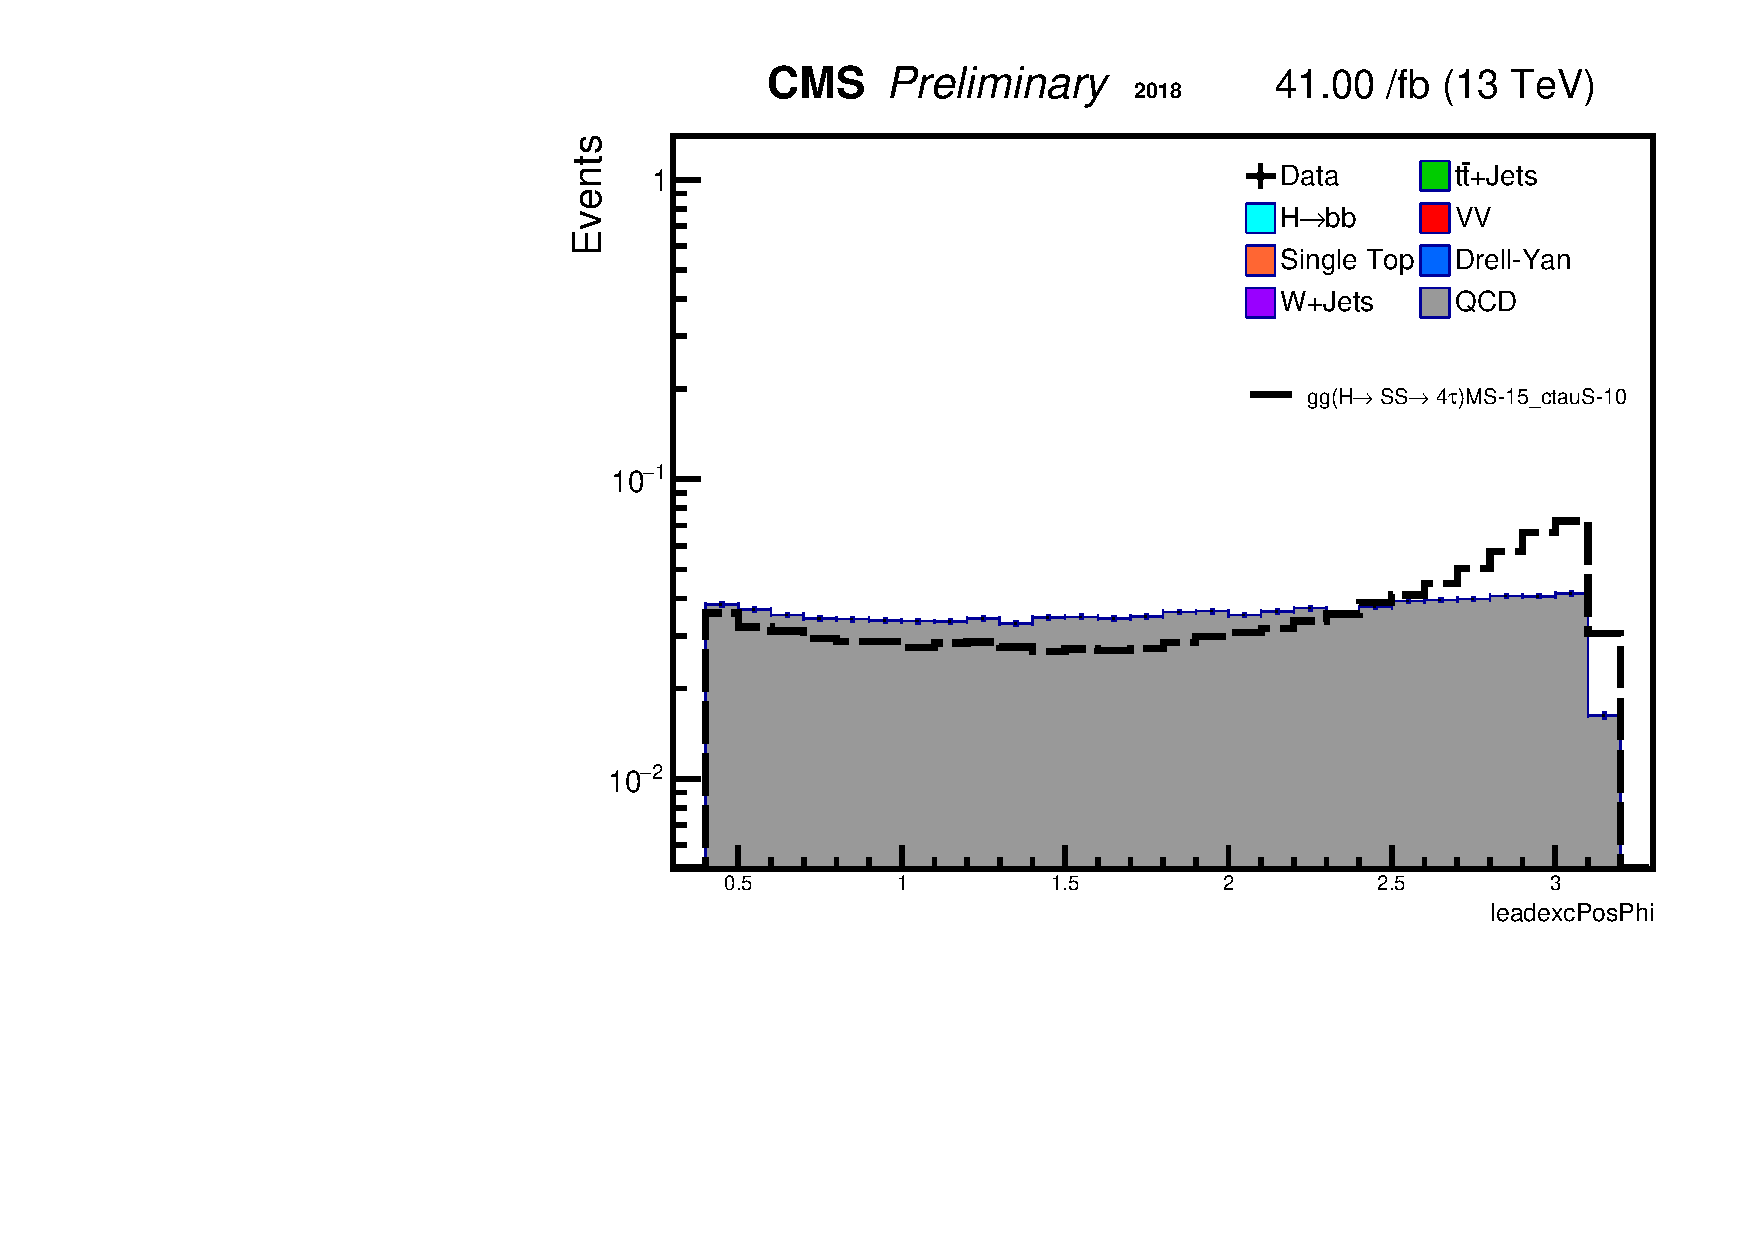
\includegraphics[width=0.47\linewidth]{figs/AnalysisNoteplot_MS-15_ctauS-10_leadexcPosPhi.pdf}
   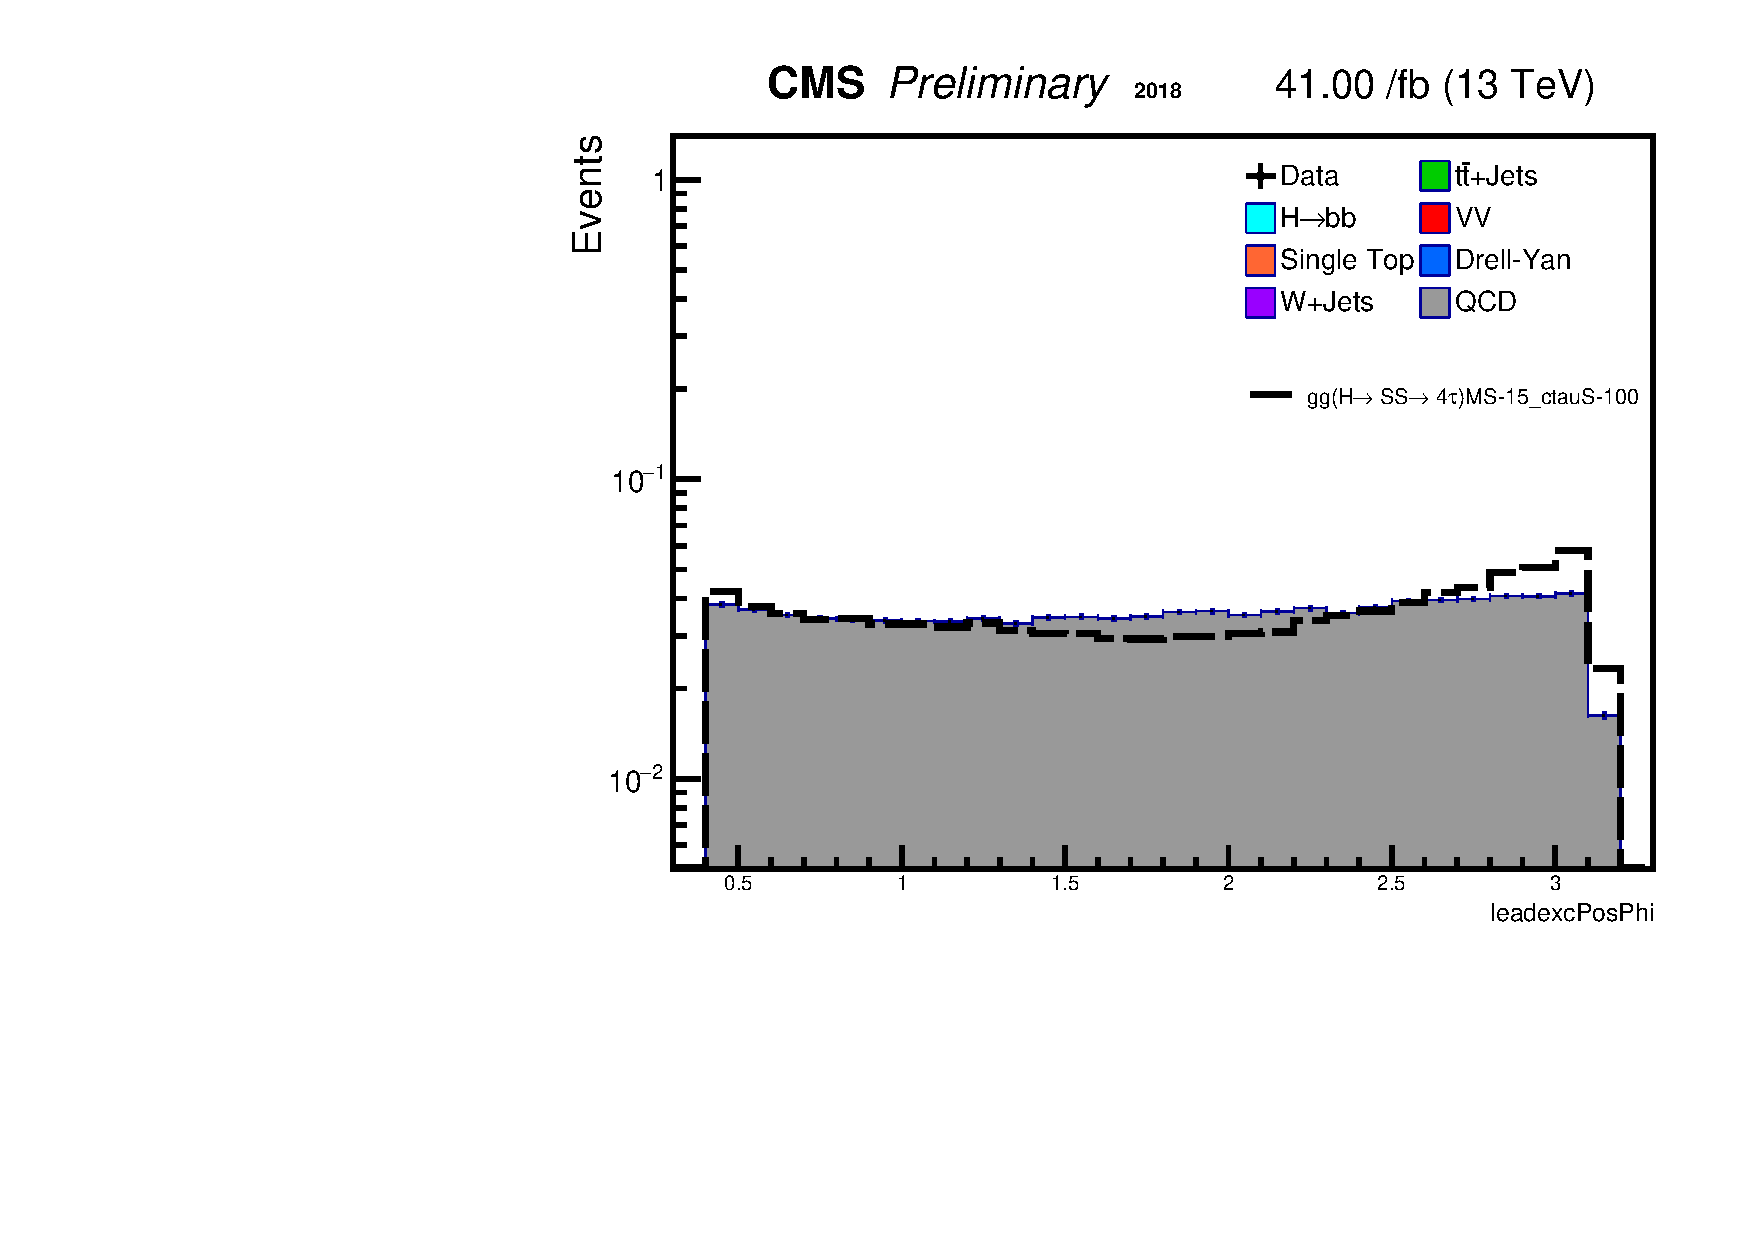
\includegraphics[width=0.47\linewidth]{figs/AnalysisNoteplot_MS-15_ctauS-100_leadexcPosPhi.pdf}
 \end{figure}








\section{Number of Annulus Tracks Associated with ROI}\label{ref:NumAnnulus}
 The tensorflow used for this analysis is trained with $p_T, \eta, \chi^{2}$, and other information of the annulus tracks (tracks that are inside ROI radius, but not fitted to vertex).
Meanwhile, an ROI's total number of annulus tracks is not a direct input for ML and tensorflow can only learn such information indirectly via annulus tracks' $p_T$.
Although having selected ROIs with high scores ($>$0.999), signal processes ROIs' number of annulus tracks show a quite different distribution from the background process.
%Figure ~\ref{fig:ANnum}
signal's high-scoring ROIs are mostly from the the exotic LLP scalar's decay into $\tau$ leptons. 
%The $\tau$ leptons have most 3 charged tracks for 12\%, and 1 charged track for 80\% of its decay mode ~\cite{willbedonelater}
Since the signal's high-score ROIs' are very well isolated, the ROI's number of annulus tracks is very low.
QCD background events, which are our dominant background, have a poor isolation quality.
Since QCD's high-scoring ROI's are poorly isolated due to QCD nature, these ROIs' numbers of annulus tracks are higher than the signal.
More precisely, QCD's high-scoring ROI's are usually from B-mesons, which have higher track multiplicity than $\tau$ leptons.


%% \begin{figure}[h!]
 \begin{figure}[h!]
   \caption{Number of tracks in the annulus cone of the leading ROI. Left plot is for MS-15\_ctauS-10mm point, whereas the right plot is for MS-15\_cauS-100mm point}
   \label{fig:ANleadSize}
   \centering
   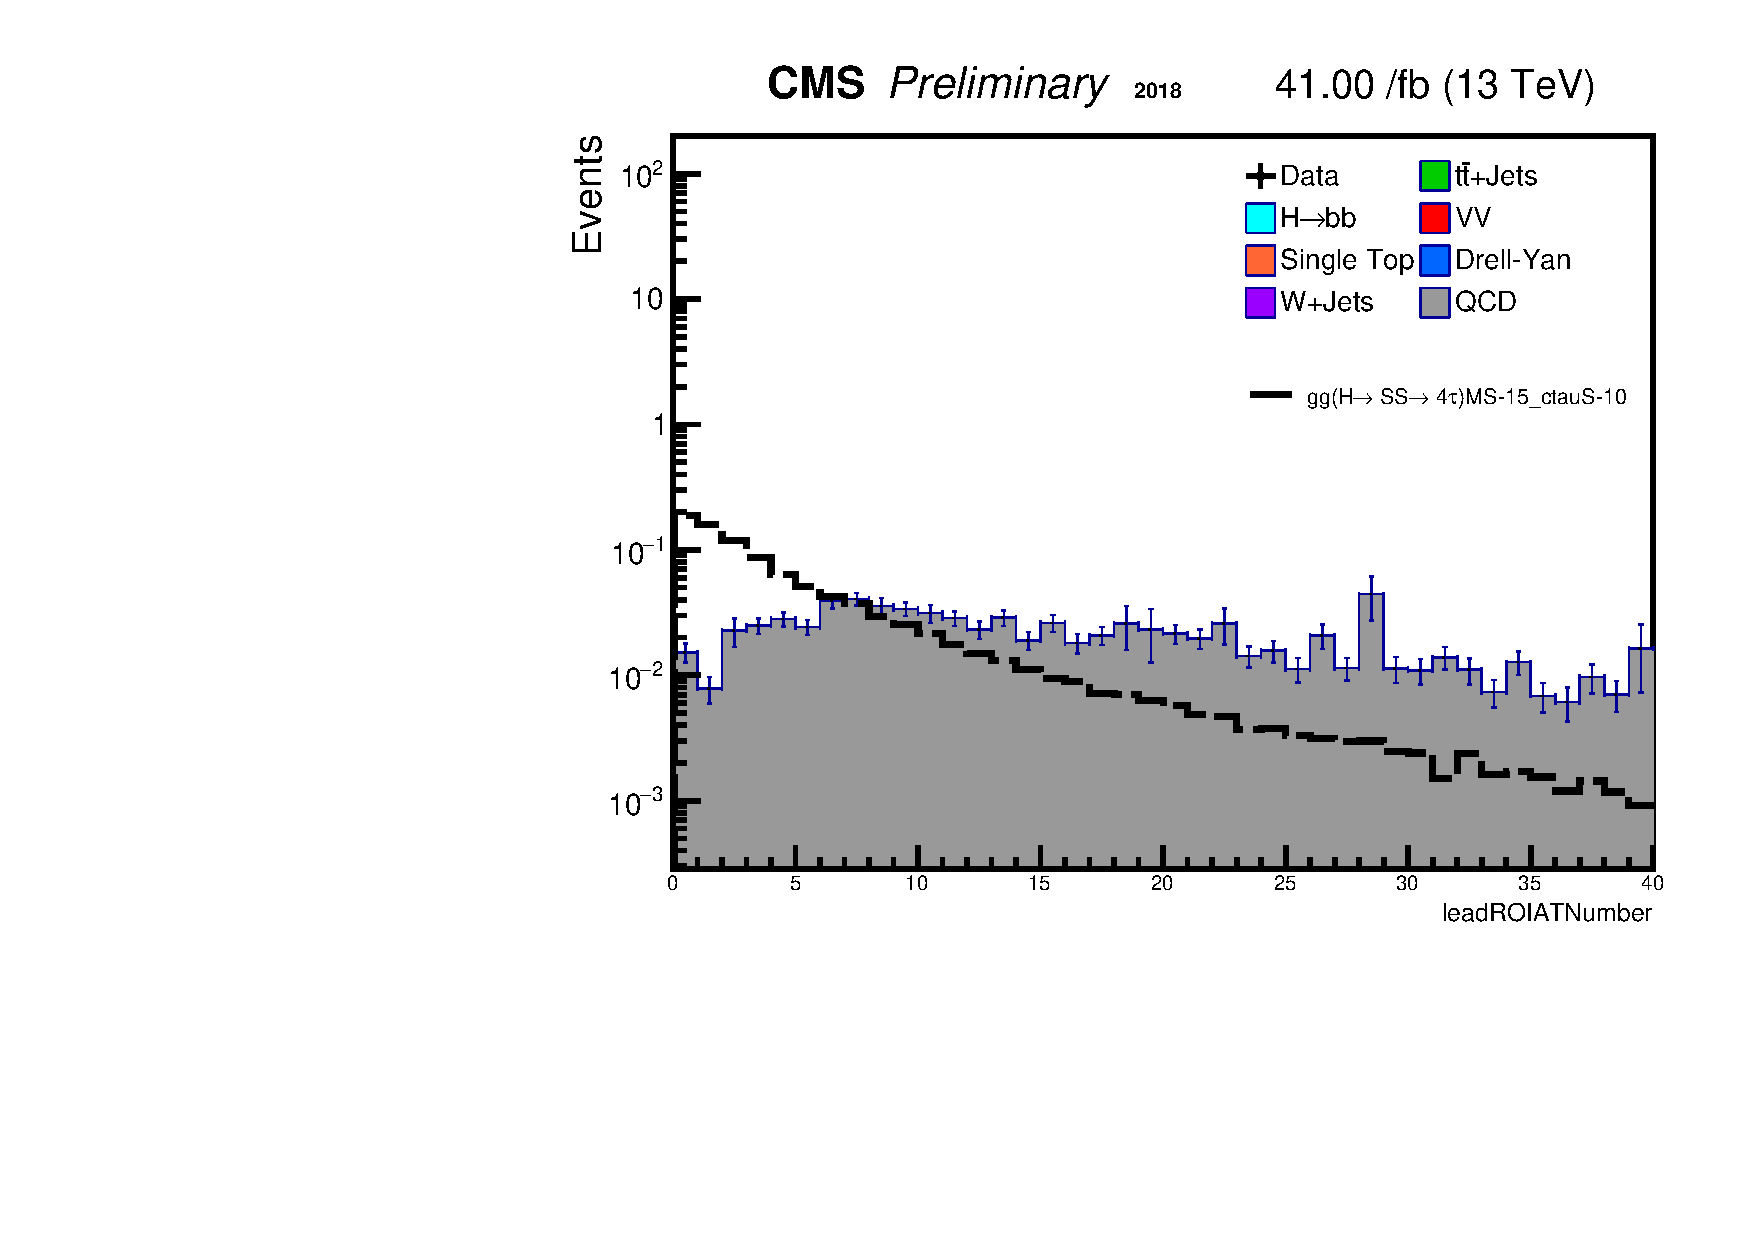
\includegraphics[width=0.47\linewidth]{figs/AnalysisNoteplot_MS-15_ctauS-10_leadROIATNumber.pdf}
   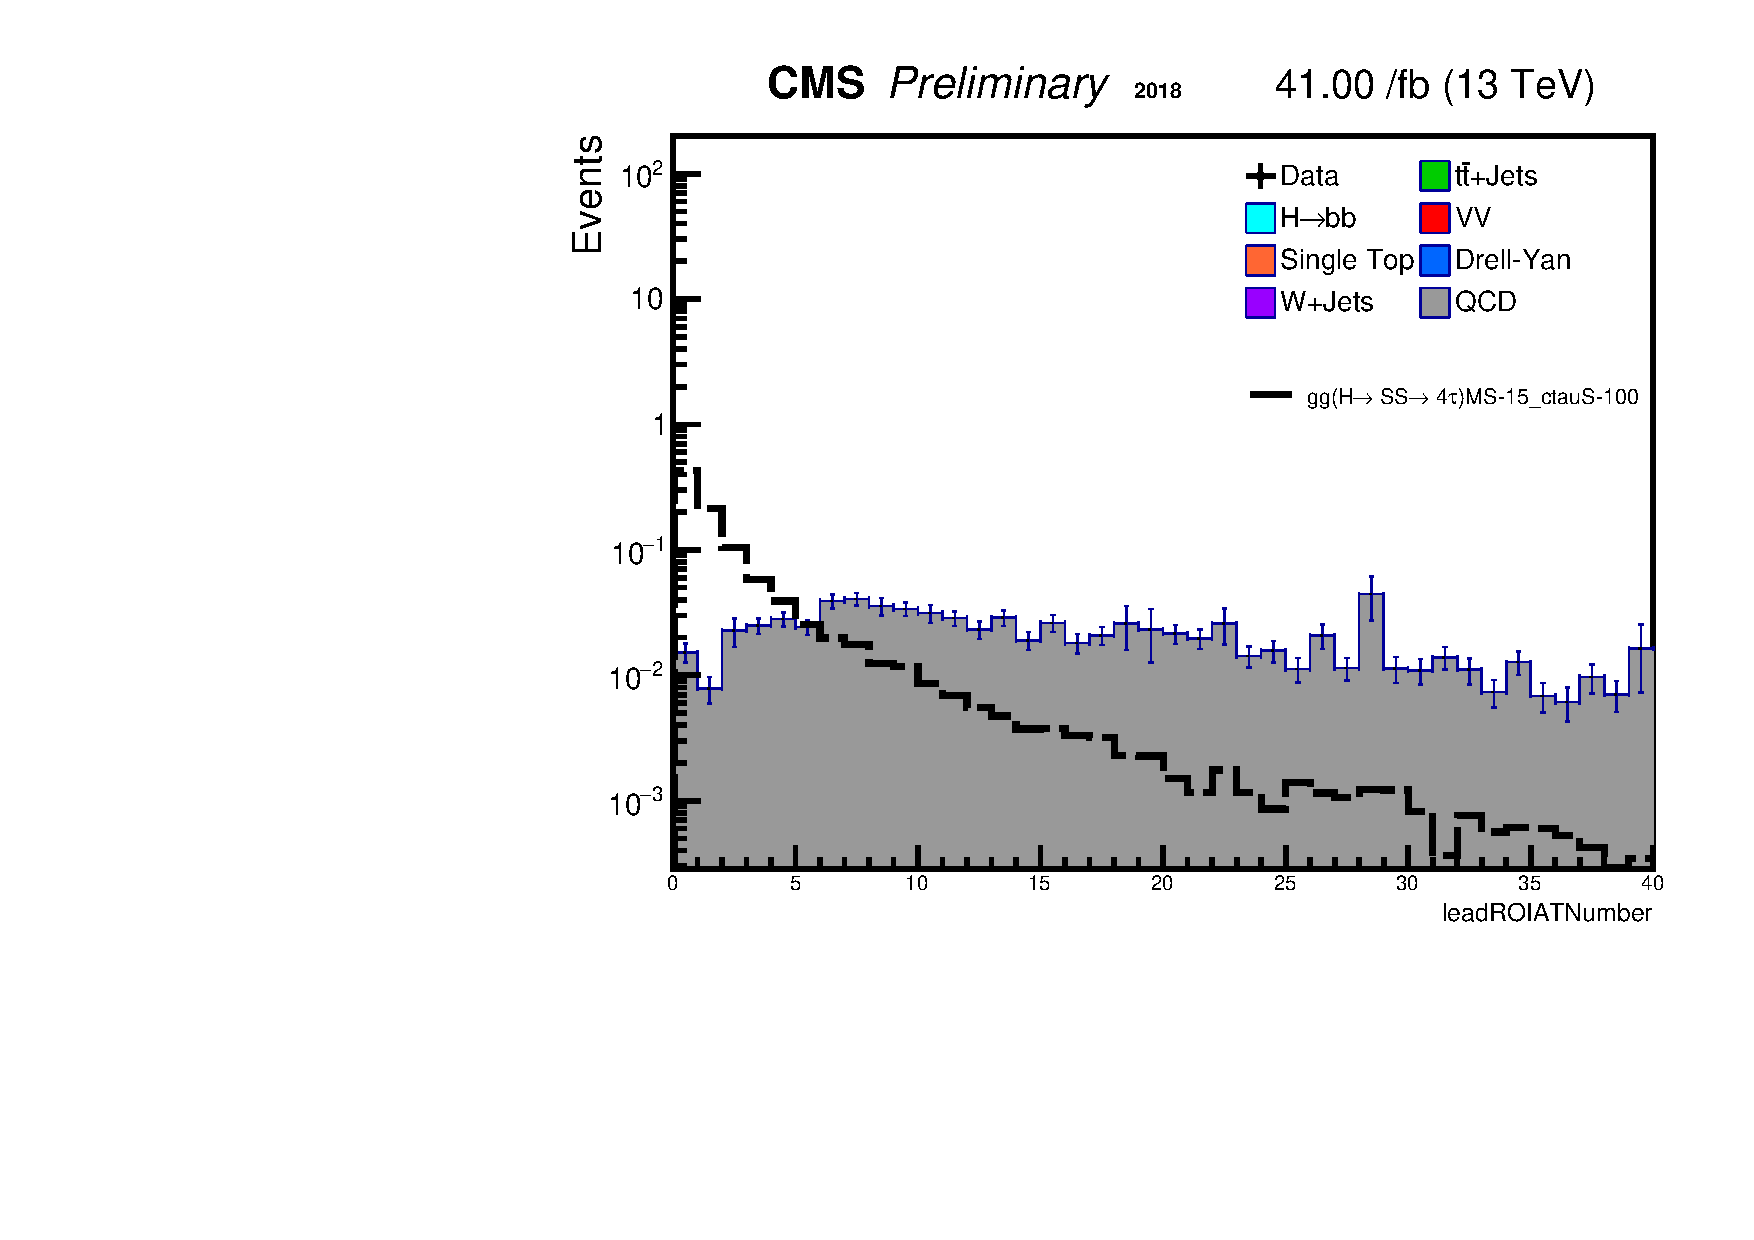
\includegraphics[width=0.47\linewidth]{figs/AnalysisNoteplot_MS-15_ctauS-100_leadROIATNumber.pdf}
 \end{figure}




\section{Isolation criteria for muons}\label{ref:muISO}
%As discussed in ~\ref{sec:NumAnnulus}, the main background for our analysis comes from QCD background events, especially from B-meson decay of QCD events with high ROI scores. 
Leptonic decay of B-meson generates muons, which trigger the B-parking trigger of the analysis.
Muons of B-meson decay have very poor isolation quality, just like ROIs formed around the B-meson decay.
In contrast, muons of $\tau$ lepton decay have better isolation quality.
In order to eliminate the dominant B-meson background from the QCD process, the analysis applies a PFISOLoose in selecting muon objects.
The precise definition of PFISOLoose is defined as below.
\begin{itemize}
  \item $(\Sigma pT(ch.had from PV)+max(0,\Sigma ET(neut.had) \Sigma ET (phot)-0.5* \Sigma pT(ch.had from PU)))/P_{T}(\mu)<0.25$
\end{itemize}

%Not only muons decayed from $\tau$ leptons with 55, 40GeV mass have a good isolation quality, but also muons of $\tau$ leptons from 15 GeV have a decent isolation quality based on gen-level $\Delta R(\tau,\bar_{\tau})$.
Some muons decayed from $\tau$ lepton with 7 GeV mass fail isolation cut, due to its poorer isolation quality from the boost.
However, it still benefits to apply the PFISOLoose cut on muons given it removes more background events than signal events.
The table below demonstrates event yield drop before and after requiring PFISOLoose cut on muons, classified by its signal and background process. 


\section{Leading muon's transverse impact parameter to PV}\label{ref:muIP}
With the B-Parking trigger, triggering muons have significant transverse displacement (impact parameter) in both background and signal processes.
However, displacement in the signal process is greater than the that of the background process.
The signal process has at minimum of c$\tau$ = 1mm, which is longer than B-meson lifetime.
Thus, triggering muon object's transverse impact parameter to PV is larger in signal process than background process.
The analysis implements a cut on this variable.


 \begin{figure}[h!]
   \caption{leading muon's transverse impact parameter value to the primary vertex. Left plot is for MS-15\_ctauS-10mm point, whereas the right plot is for MS-15\_cauS-100mm point}
   \label{fig:leadmuIP}
   \centering
   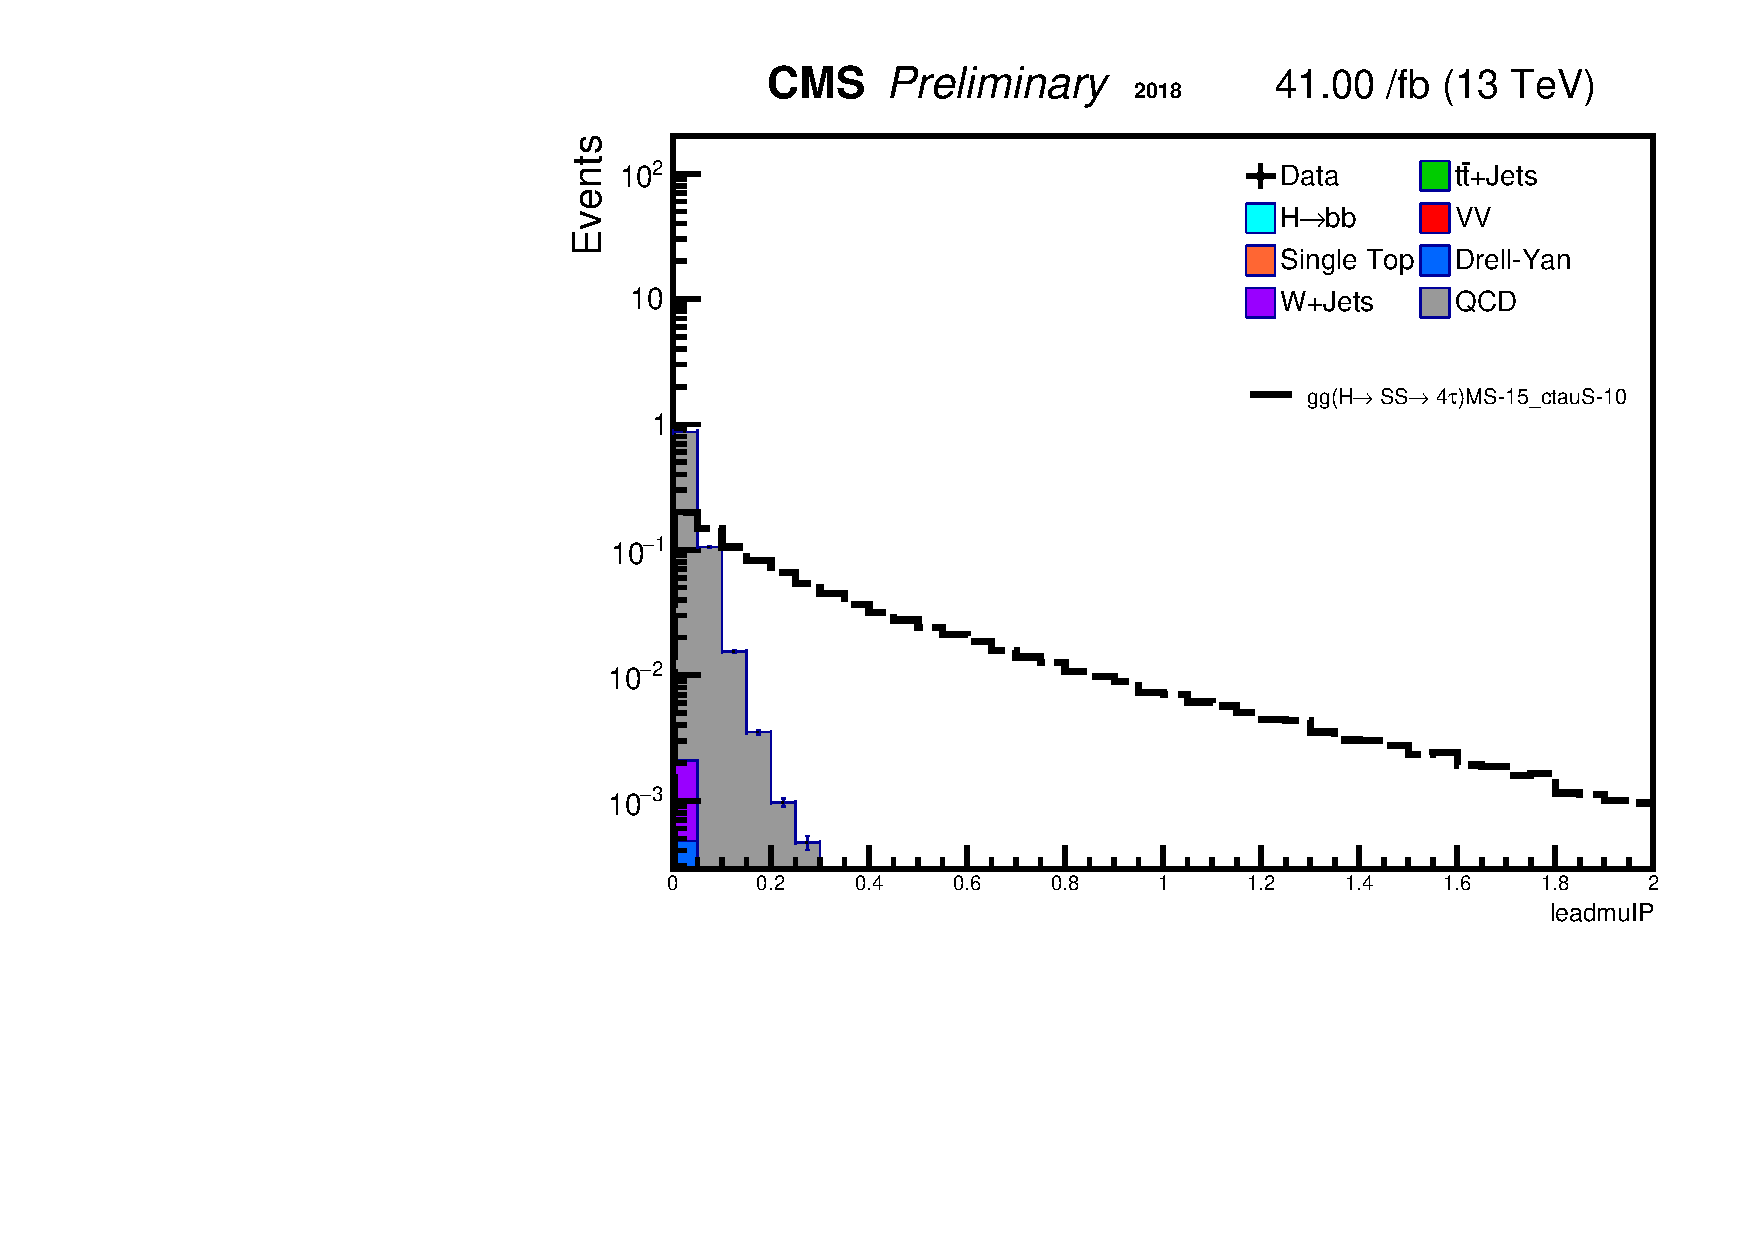
\includegraphics[width=0.47\linewidth]{figs/AnalysisNoteplot_MS-15_ctauS-10_leadmuIP.pdf}
   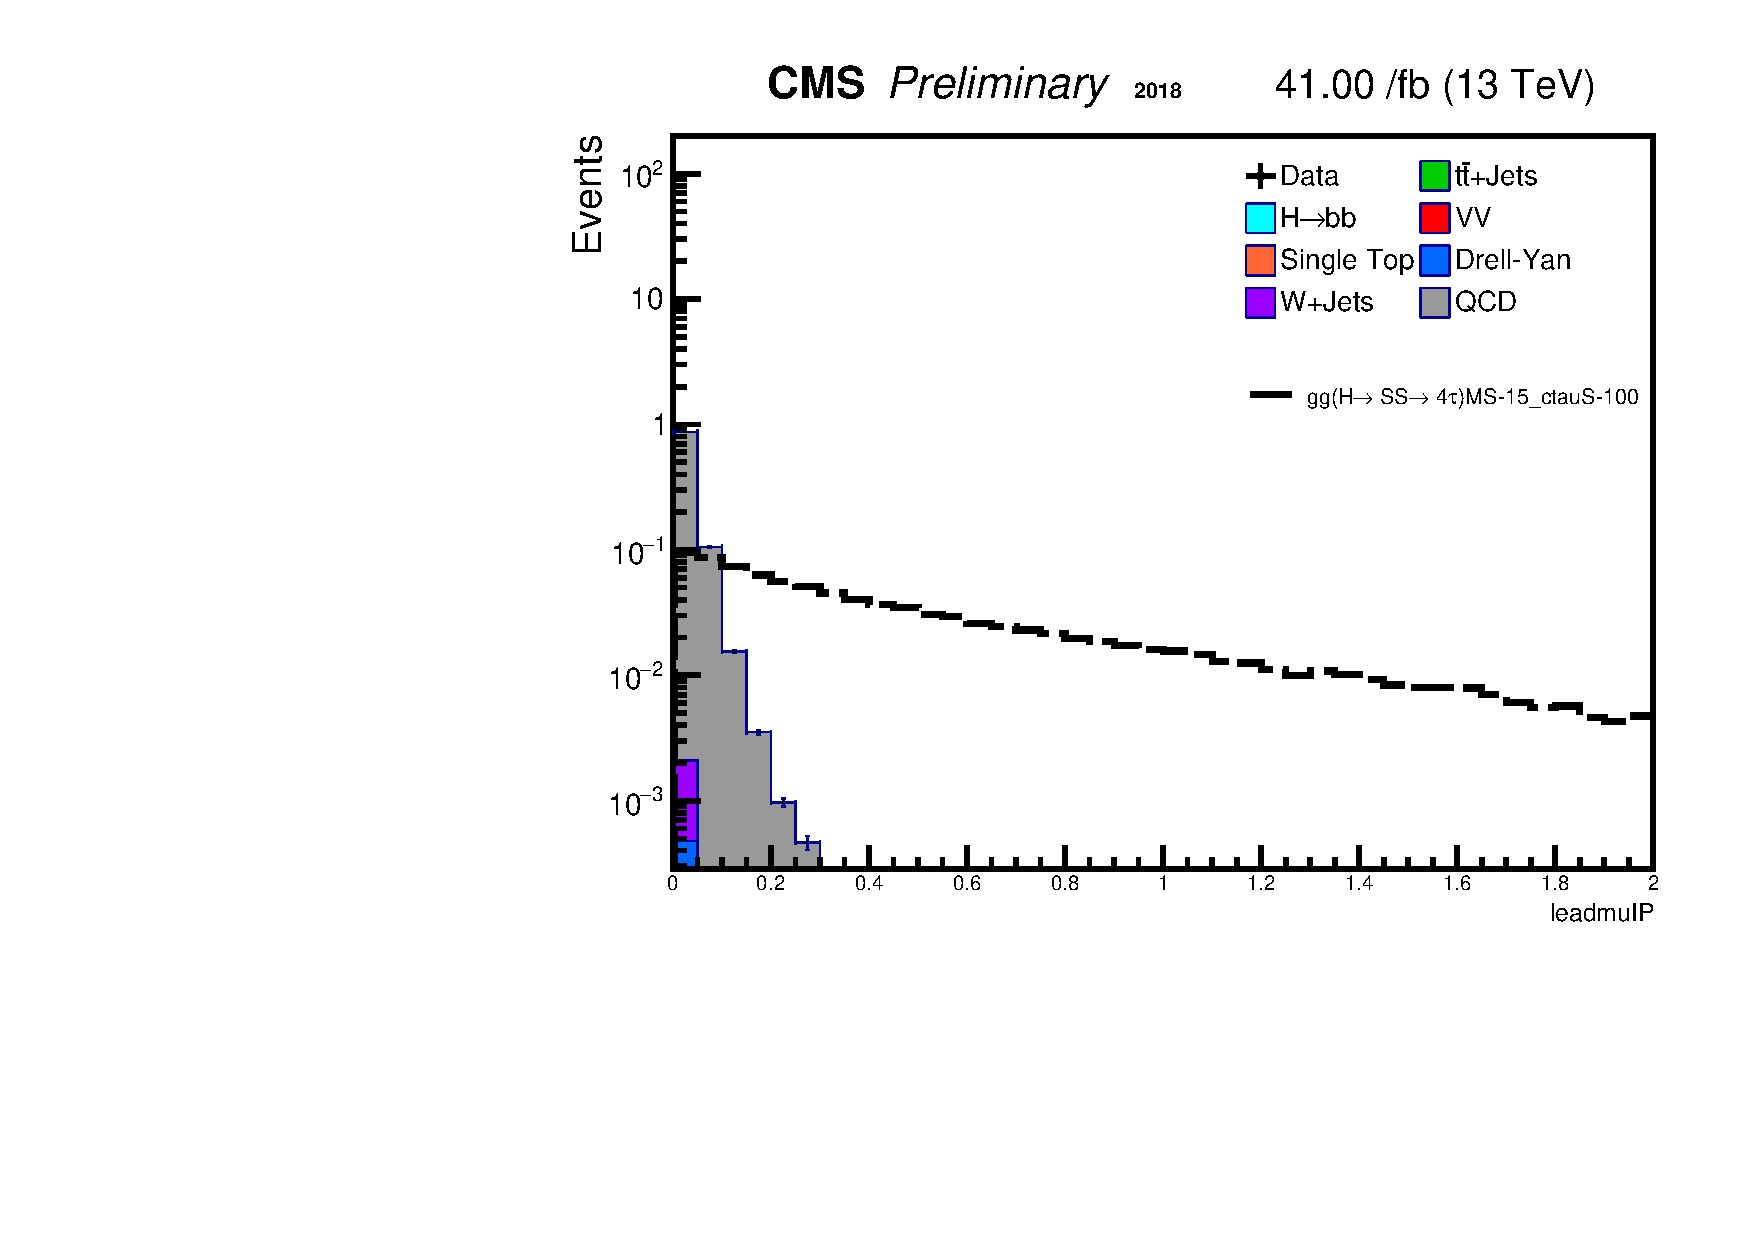
\includegraphics[width=0.47\linewidth]{figs/AnalysisNoteplot_MS-15_ctauS-100_leadmuIP.pdf}
 \end{figure}


\section{DeltaR(ROI, jet)}\label{ref:jetdR}
$\tau$ leptons of the signal process can also decay hadronically, while only one of the $\tau$ leptons decay muonically to trigger B parking trigger.
When $\tau$ leptons decay hadronically, its decay shower can get clustered in the calorimeter, and reconstructed as a jet.
Given the $\tau$ lepton's on-shell mass is a fixed value, $\tau$ lepton and its hadronic decay products (to-be clustered into a jet) have a specific kinematic phase space.
Thus, the $\Delta$ R(ROI, jet) has a distribution with a peak at a certain value (around 0.3-0.6).
Meanwhile, the QCD backround has a different distribution shape.
Given the hadronic nature of the process, jet multiplicity is high. 
Higher jet multiplicity makes the $\Delta$ R(ROI,jet) value to have a rather randomized value, resulting in a flat distribution. 

 \begin{figure}[h!]
   \caption{Delta R(Jet, leadingROI). Left plot is for MS-15\_ctauS-10mm point, whereas the right plot is for MS-15\_cauS-100mm point}
   \label{fig:ANleadSize}
   \centering
   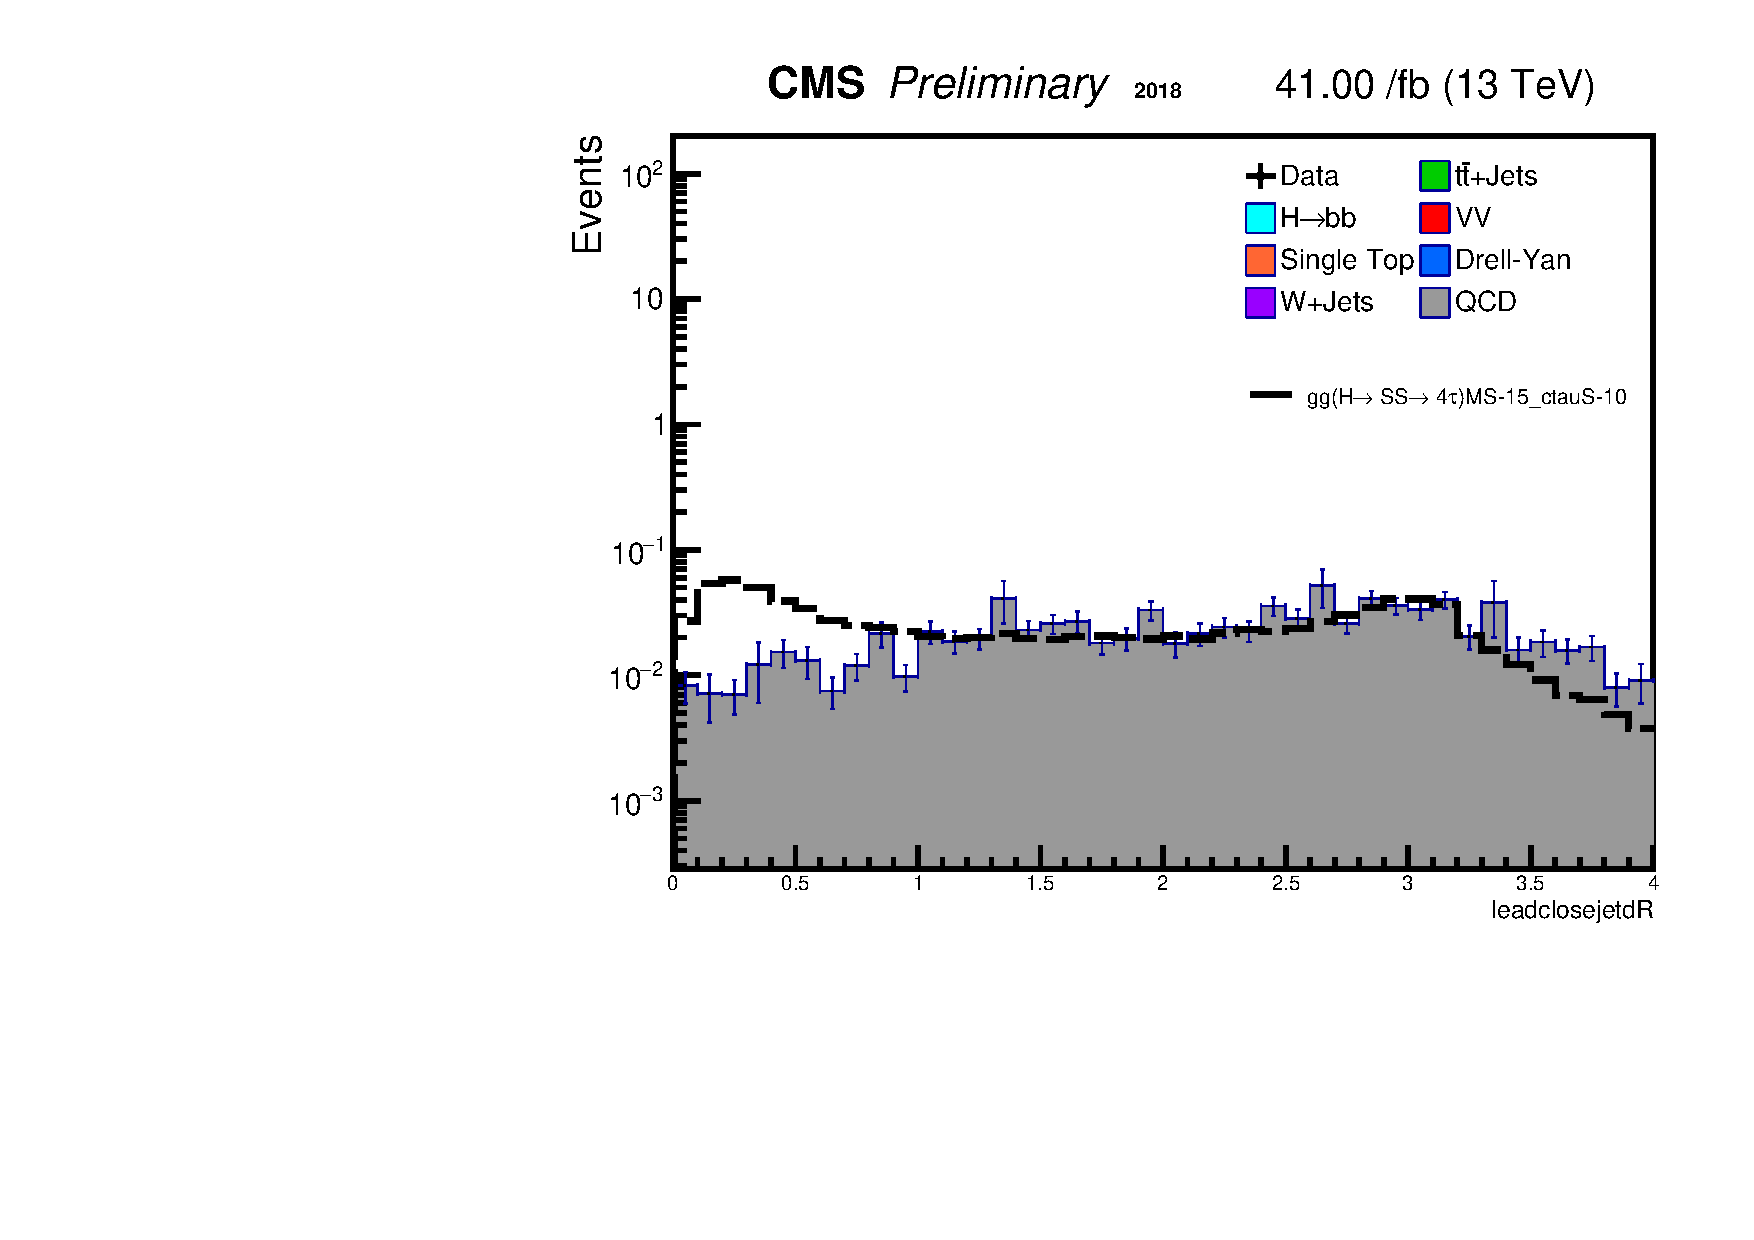
\includegraphics[width=0.47\linewidth]{figs/AnalysisNoteplot_MS-15_ctauS-10_leadclosejetdR.pdf}
   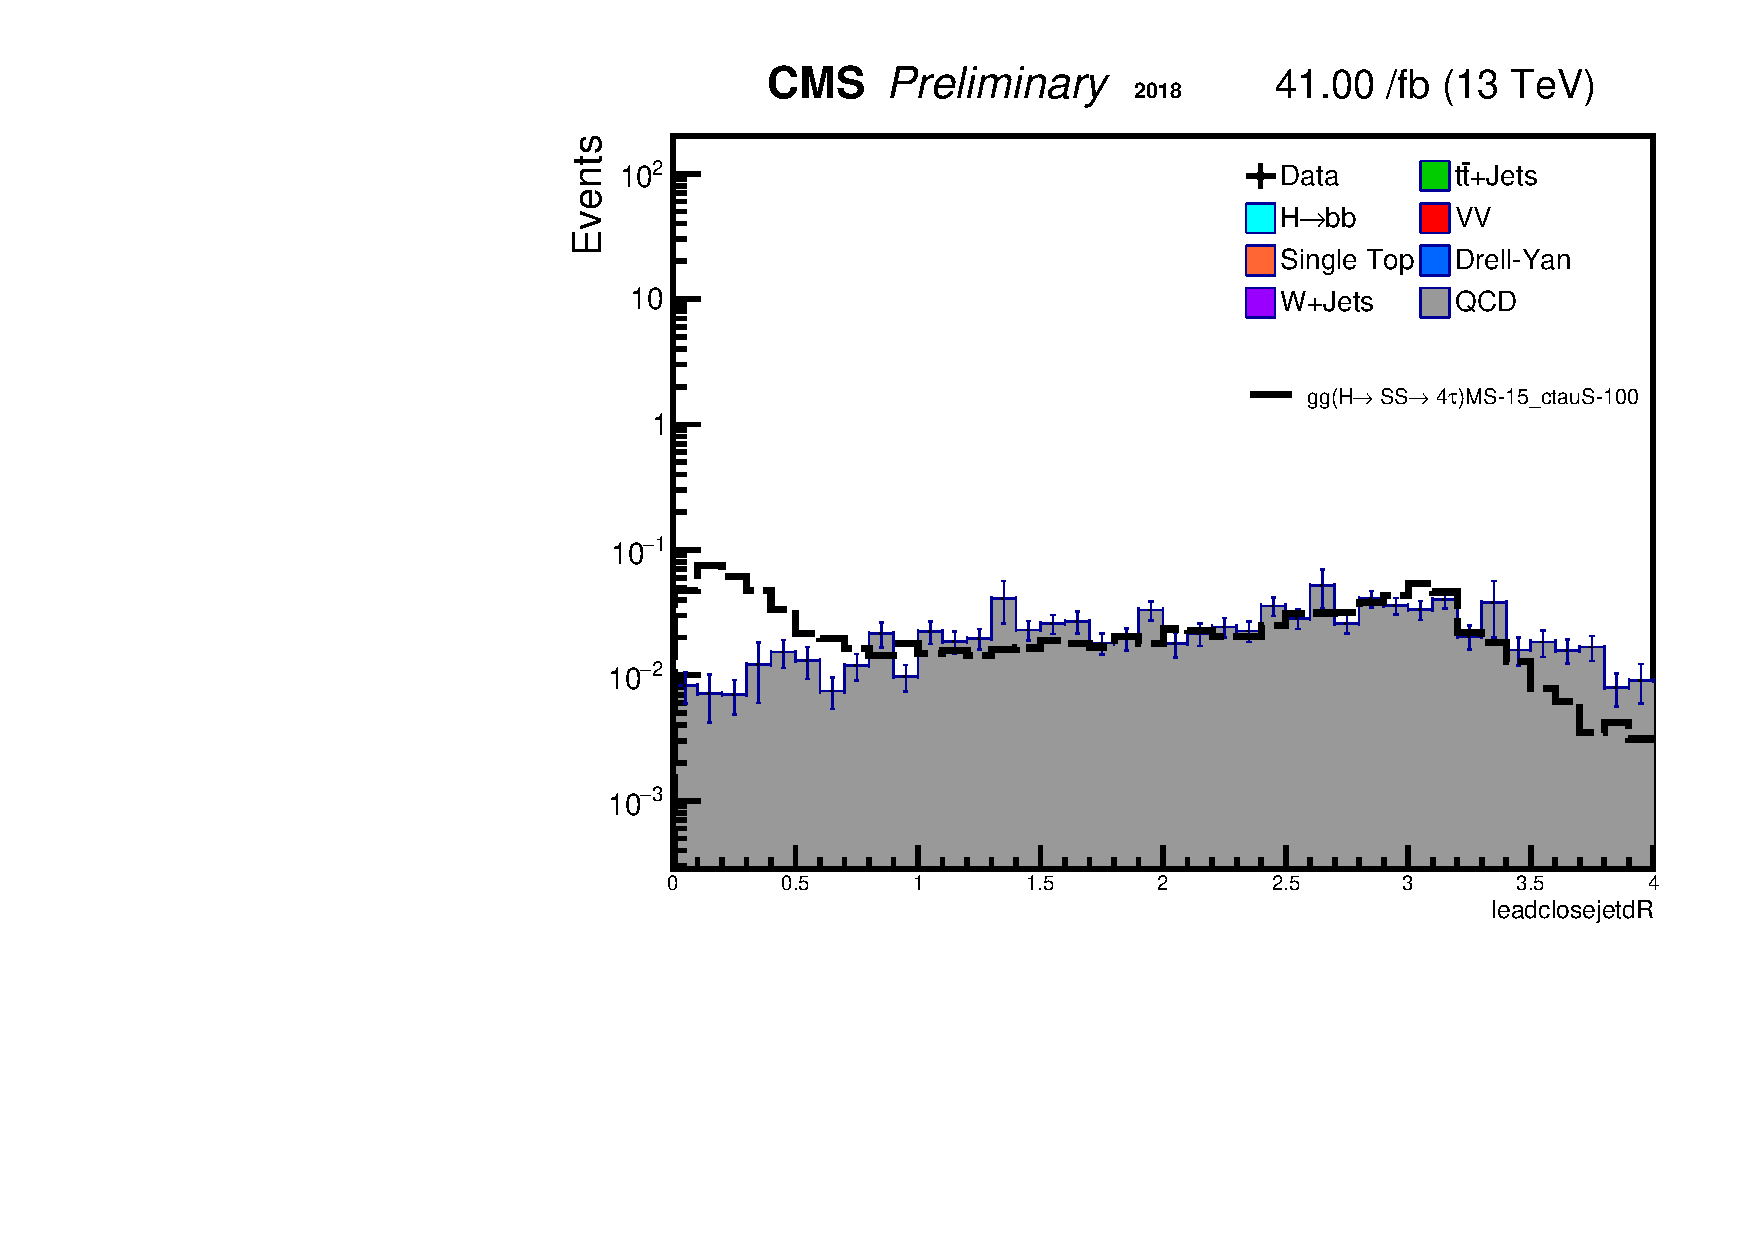
\includegraphics[width=0.47\linewidth]{figs/AnalysisNoteplot_MS-15_ctauS-100_leadclosejetdR.pdf}
 \end{figure}



%% \begin{figure}[h!]
%%   \caption{Trigger turn-on curves for the 17 MuonEG HLT path. Leading \pt
%%   lepton (left) and subleading \pt lepton (right).}
%%   \label{fig:17_trigger_turnon_mueg}
%%   \centering
%%   \includegraphics[width=0.40\linewidth]{figs/2017_TTOCEMu_ElePt.png}
%%   \includegraphics[width=0.40\linewidth]{figs/2017_TTOCEMu_MuPt.png}
%% \end{figure}


%% \begin{figure}[h!]
%%   \caption{Trigger turn-on curves for the 17 MuonEG HLT path. Leading \pt
%%   lepton (left) and subleading \pt lepton (right).}
%%   \label{fig:17_trigger_turnon_mueg}
%%   \centering
%%   \includegraphics[width=0.40\linewidth]{figs/2017_TTOCEMu_ElePt.png}
%%   \includegraphics[width=0.40\linewidth]{figs/2017_TTOCEMu_MuPt.png}
%% \end{figure}
%% \begin{figure}[h!]
%%   \caption{Trigger turn-on curves for the 16 DoubleElectron HLT paths. Leading \pt
%%   lepton (left) and subleading \pt lepton (right).}
%%   \label{fig:16_trigger_turnon_dielectron}
%%   \centering
%%   \includegraphics[width=0.40\linewidth]{figs/2016_TTOCEle1Pt.png}
%%   \includegraphics[width=0.40\linewidth]{figs/2016_TTOCEle2Pt.png}
%% \end{figure}
%%
%% \begin{figure}[h!]
%%   \caption{Trigger Efficiency for the 16 DoubleElectron HLT paths. Leading and subleading
%%   lepton vs \pt (left) and $\eta$ (right).}
%%   \label{fig:16_trigger_turnon__twoD_dielectron}
%%   \centering
%%   \includegraphics[width=0.40\linewidth]{figs/2016_TTOC_Ele23Ele12_DElePt.png}
%%   \includegraphics[width=0.40\linewidth]{figs/2016_TTOC_Ele23Ele12_DEleEta.png}
%% \end{figure}
%%
%% \begin{figure}[h!]
%%   \caption{Trigger turn-on curves for the 16 DoubleMuon HLT paths. Leading \pt
%%   lepton (left) and subleading \pt lepton (right).}
%%   \label{fig:16_trigger_turnon_dimuon}
%%   \centering
%%   \includegraphics[width=0.40\linewidth]{figs/2016_TTOCMu1Pt.png}
%%   \includegraphics[width=0.40\linewidth]{figs/2016_TTOCMu2Pt.png}
%% \end{figure}
%%
%% \begin{figure}[h!]
%%   \caption{Trigger Efficiency for the 16 DoubleMuon HLT paths. Leading  and subleading
%%   lepton vs \pt (left) and $\eta$ (right).}
%%   \label{fig:16_trigger_turnon__twoD_dimuon}
%%   \centering
%%   \includegraphics[width=0.40\linewidth]{figs/2016_TTOC_Mu17Mu8_DMuPt.png}
%%   \includegraphics[width=0.40\linewidth]{figs/2016_TTOC_Mu17Mu8_DMuEta.png}
%% \end{figure}
%%
%%
%% \begin{figure}[h!]
%%   \caption{Trigger turn-on curves for the 16 MuonEG HLT path. Leading \pt
%%   lepton (left) and subleading \pt lepton (right).}
%%   \label{fig:16_trigger_turnon_mueg}
%%   \centering
%%   \includegraphics[width=0.40\linewidth]{figs/2016_TTOCEMu_ElePt.png}
%%   \includegraphics[width=0.40\linewidth]{figs/2016_TTOCEMu_MuPt.png}
%% \end{figure}
%%
%% \begin{figure}[h!]
%%   \caption{Trigger turn-on curves for the 17 DoubleElectron and DoubleMuon HLT paths. Electron \pt
%%   (left) and Muon \pt lepton (right).}
%%   \label{fig:17_trigger_turnon_dielectron_and_dimuon}
%%   \centering
%%   \includegraphics[width=0.40\linewidth]{figs/2017_TTOCEle1Pt.png}
%%   \includegraphics[width=0.40\linewidth]{figs/2017_TTOCMu1Pt.png}
%% \end{figure}
%%
%% \begin{figure}[h!]
%%   \caption{Trigger Efficiency for the 17 DoubleElectron HLT paths. Leading and subleading
%%   lepton vs \pt (left) and $\eta$ (right).}
%%   \label{fig:17_trigger_turnon__twoD_dielectron}
%%   \centering
%%   \includegraphics[width=0.40\linewidth]{figs/2017_TTOC_Ele23Ele12_DElePt.png}
%%   \includegraphics[width=0.40\linewidth]{figs/2017_TTOC_Ele23Ele12_DEleEta.png}
%% \end{figure}
%%
%%
%% \begin{figure}[h!]
%%   \caption{Trigger Efficiency for the 17 DoubleMuon HLT paths. Leading  and subleading
%%   lepton vs \pt (left) and $\eta$ (right).}
%%   \label{fig:17_trigger_turnon__twoD_dimuon}
%%   \centering
%%   \includegraphics[width=0.40\linewidth]{figs/2017_TTOC_Mu17Mu8_DMuPt.png}
%%   \includegraphics[width=0.40\linewidth]{figs/2017_TTOC_Mu17Mu8_DMuEta.png}
%% \end{figure}
%%
%%
%% \begin{figure}[h!]
%%   \caption{Trigger turn-on curves for the 17 MuonEG HLT path. Leading \pt
%%   lepton (left) and subleading \pt lepton (right).}
%%   \label{fig:17_trigger_turnon_mueg}
%%   \centering
%%   \includegraphics[width=0.40\linewidth]{figs/2017_TTOCEMu_ElePt.png}
%%   \includegraphics[width=0.40\linewidth]{figs/2017_TTOCEMu_MuPt.png}
%% \end{figure}
%
%\clearpage
%\section{Search Regions}\label{sec:searhregion}
%
%\begin{itemize}
%  \item $\geq$ 1 good primary vertex
%  \item One \dilepton pair with 70 GeV $<$ m(\dilepton) $<$ 110 GeV and \pt(\dilepton) $>$ 100 GeV
%  \item No additional leptons with \pt $\geq$ 15 GeV
%  \item $\geq$ 1 jet
%\end{itemize}
%
%Where $\ell = e, \mu$. We refer to the subsets of the search region with
%$\ell = e$ and  $\ell = \mu$ as \twoelezh and \twomuzh, respectively.
%
%The leading lepton in the opposite-sign same-flavor (OSSF) pair is required to have \pt $\geq$ 25 GeV,
%while the subleading lepton is required to have \pt $\geq$ 15 GeV.
%These cuts were chosen to be near the plateau of the trigger efficiency.
%
%The \pt cut on the OSSF lepton pair was optimized for this analysis.
%It is well known from standard model searches for associated Higgs production that the Z spectrum
%in associated production is harder than that of background. Figures~\ref{fig:zpt}-\ref{fig:zpt2} show
%the di-lepton transverse momentum distribution.
%Figure \ref{fig:ptossf} shows this with unit normalized \pt(\dilepton) distributions of the total background
%and an example signal according to simulation.
%We find that a \pt(\dilepton) threshold of approximately 100~\GeV reaches a near
% optimal sensitivity, thus we select a \pt(\dilepton) $>$ 100~\GeV to define the
%  search region ($\mathrm{high-\pt}$).
%This was found to be true for all scalar masses within the 10-100~\mm lifetime range.
%This is shown for an example signal in Figure \ref{fig:ptossfopt}. Sec.~\ref{sec:signaleff}
%has more details on the signal efficiency cut-flow yields in the different search
% and control regions.
%
%
%\begin{figure}[h!]
%  \caption{\pt(\dilepton) distributions of the total background from MC and data in 2016.
%  (Left) the distribution for the $\mu^+\mu^-$ and (right) $e^+e^-$ channels.}
%  \label{fig:zpt}
%  \centering
%  \includegraphics[width=0.45\linewidth]{figs/v6/2016_TwoMuOffZ_AOD_dileptonNewB_Pt_GH.pdf}
%  \includegraphics[width=0.45\linewidth]{figs/v6/2016_TwoEleOffZ_AOD_dileptonNewB_Pt_GH.pdf}
%\end{figure}
%\begin{figure}[h!]
%  \caption{\pt(\dilepton) distributions of the total background from MC and data in 2017.
%  (Left) the distribution for the $\mu^+\mu^-$ and (right) $e^+e^-$ channels.}
%  \label{fig:zpt2017}
%  \centering
%  \includegraphics[width=0.45\linewidth]{figs/v6/2017_TwoMuOffZ_AOD_dileptonNewB_Pt.pdf}
%  \includegraphics[width=0.45\linewidth]{figs/v6/2017_TwoEleOffZ_AOD_dileptonNewB_Pt.pdf}
%\end{figure}
%\begin{figure}[h!]
%  \caption{\pt(\dilepton) distributions of the total background from MC and data in 2018.
%  (Left) the distribution for the $\mu^+\mu^-$ and (right) $e^+e^-$ channels.}
%  \label{fig:zpt2}
%  \centering
%  \includegraphics[width=0.45\linewidth]{figs/v10/2018_TwoMuOffZ_AOD_dileptonNewB_Pt.pdf}
%  \includegraphics[width=0.45\linewidth]{figs/v10/2018_TwoEleOffZ_AOD_dileptonNewB_Pt.pdf}
%\end{figure}
%\begin{figure}[h!]
%  \caption{\pt(\dilepton) distributions of the total background from MC and data corresponding to the target
%  luminosity used in the analysis and combine ee and $\mu\mu$-channels. }
%  \label{fig:zpt2}
%  \centering
%  %\includegraphics[width=0.45\linewidth]{figs/v10/TwoMuOffZ_AOD_dileptonNewB_Pt.pdf}
%  \includegraphics[width=0.45\linewidth]{figs/v10/eemumu_dileptonNewB_Pt.png}
%\end{figure}
%
%
%
%\begin{figure}[h!]
%  \caption{Unit normalized \pt(\dilepton) distributions of the total background and an example signal in simulation.
%    The event selection is that of the \twomuzh search region without the  \pt(\dilepton) cut
%    with an additional requirement of at least one displaced-jet tag.
%    The example signal has a scalar mass of 40 GeV and a proper-lifetime of 10 mm.
%  }
%  \label{fig:ptossf}
%  \centering
%  \includegraphics[width=0.60\linewidth]{figs/ptossf.pdf}
%\end{figure}
%
%
%\begin{figure}[h!]
%  \caption{Sensitivity quantified by $S$/$\sqrt{S+B}$ as a function of \pt(\dilepton) threshold for one example signal.
%    The event selection is that of the \twomuzh search region without the  \pt(\dilepton) cut
%    with an additional requirement of at least one displaced-jet tag.
%    The example signal has a scalar mass of 40 GeV and a lifetime of 10 mm, but the result does not vary strongly with either.
%}
%  \label{fig:ptossfopt}
%  \centering
%  \includegraphics[width=0.60\linewidth]{figs/ptossfopt.pdf}
%\end{figure}
%
%
%
%The MC expected distribution of the displaced-jet tag multiplicity (\NTAGS)
%for SM background and signals, in the \twollzh search region, are shown in
%Figure~\ref{fig:ntag_cp_2020_2}.
%\NTAGS depends on the scalar mass due to the merging of its decay products
%(see right panel of Figure~\ref{fig:scalarpt}).
%Therefore, we expect this search to have different sensitivities for different scalar mass
%scenarios.
%%to peform a generic search for a range of scalar masses,
%%we perform the search in the tag multiplicity distribution.
%
%% \begin{figure}[h!]
%%   \caption{\NTAGS distributions in the \twoelezh search region (left) and \twomuzh search region (right).}
%%   \label{fig:zhntag}
%%   \centering
%%   \includegraphics[width=0.47\linewidth]{figs/TwoEleZH_nSelectedAODCaloJetTag_log.pdf}
%%   \includegraphics[width=0.47\linewidth]{figs/TwoMuZH_nSelectedAODCaloJetTag_log.pdf}
%% \end{figure}
%\begin{figure}[h!]
%  \caption{\NTAGS distribution in the \twollzh search region (left) and \twolldy
%  control region (right). Here the BR($H\rightarrow SS \rightarrow bbbb$) is assumed to be 20\% for the signal.}
%  \label{fig:ntag_cp_2020_2}
%  \centering
%  \includegraphics[width=0.47\linewidth,valign=t]{figs/v12/ZH_nSelectedAODCaloJetTag_log.png}
%  \includegraphics[width=0.47\linewidth,valign=t]{figs/v12/DY_nSelectedAODCaloJetTag_log.png}
%
%\end{figure}
%
%
%As can be seen in Figure~\ref{fig:ntag_cp_2020_2}, the largest background is Z bosons decaying to leptons,
% that is \DY and $Z\gamma$ events -- with the former clearly dominating.
%The second largest background is events with top quarks, both $t\bar{t}$ and
% single top, hereafter referred to as top background.
%The single top background is dominated by the $tW$ channel as these events can
%produce an OSSF pair passing the search region cuts when the two W bosons
%present in these events (the W from the hard interaction, as well as the one
%from the top-quark) decay leptonically. The top background is dominated by $t\bar{t}$ production.
%The other backgrounds are a small fraction of the total.
%In the 1-tag bin, for example, the Z background is roughly 93\% of the total,
%the top backgrounds is roughly 5\% of the total, and the other backgrounds are roughly 2\% of the total.
%In the 2-tag bin, the MC statistics are limited and yields have an uncertainty
%of about 50~\%, but assuming the central values, the background composition is very similar to that of the 1-tag bin.
%
%\section{Control Regions}\label{sec:controlregion}
%
%We use control regions to perform data-driven estimates of the two largest SM
%backgrounds -- the \Z and top backgrounds.
%Here we define the control regions dedicated to estimate these two SM backgrounds.
%The rest of the backgrounds ($\sim$3~\%), hereafter referred to as
%\textbf{other backgrounds}, will be taken directly from MC simulation.
%
%\subsection{\Z Control Regions}
%
%The control region dominated by the Z background is formed
%by identical requirements as the search region with the exception of an \textbf{inverted} \ptossf cut.
%Similar to the search regions, the event level requirement for the control region are::
%\begin{itemize}
%  \item $\geq$ 1 good primary vertex
%  \item One \dilepton pair with 70 GeV $<$ m(\dilepton) $<$ 110 GeV and \pt(\dilepton) $<$ 100 GeV
%  \item No additional leptons with \pt $\geq$ 15 GeV
%  \item $\geq$ 1 jet
%\end{itemize}
%
%Where $\ell = e, \mu$. We refer to the subsets of the control region with
%$\ell = e$ and $\ell = \mu$ as \twoeledy and \twomudy, respectively.
%%We refer to the control region with $\ell = e$ as \textbf{\twoeledy}
%%and the control region with $\ell = \mu$ as \textbf{\twomudy}.
%
%The MC expected distribution and the observed data for the displaced-jet
% tag multiplicity (\NTAGS) distribution in the \twolldy control region is shown in Figure~\ref{fig:ntag_cp_2020_2} 
%(right).
%Contamination in the control region from processes other than the \Z backgound are
%accounted for in the global fit signal extraction procedure as discussed in Section~\ref{sec:estimate}.
%We note that the signal contribution in these regions is small,
%and therefore we do not blind this region in data.
%
%%Don't think we need this one anymore
%%\begin{figure}[h!]
%%  \caption{\NTAGS distributions in the \twoeledy control region (left) and \twomudy control region (right).}
%%  \label{fig:dyntag}
%%  \centering
%%  \includegraphics[width=0.47\linewidth]{figs/TwoEleDY_nSelectedAODCaloJetTag_log.pdf}
%%  \includegraphics[width=0.47\linewidth]{figs/TwoMuDY_nSelectedAODCaloJetTag_log.pdf}
%%\end{figure}
%
%
%
%\subsection{Top Control Regions}
%
%Control regions that are dominated by the $t\bar{t}$ and single-top (top) backgrounds are formed
%by changing the OSSF requirement to an opposite-sign different-flavor (OSDF) requirement.
%Concretely, we require \emu where $(\ell,\ell')$ = $(e,\mu)$ or $(\mu,e)$.
%We define two top-dominated control regions -- one in the high dilepton \pt range of the search region,
%and the other in the low dilepton \pt range of the Z background control regions.
%
%%The high dilepton \pt top control region cuts are therefore:
%%\begin{itemize}
%%  \item $\geq$ 1 good primary vertex
%%  \item One \emu pair with 70 GeV $<$ m(\emu) $<$ 110 GeV and \pt(\emu) $>$ 100 GeV
%%  \item No additional leptons with \pt $\geq$ 15 GeV
%%  \item $\geq$ 1 jet
%%\end{itemize}
%%We refer to this control region as \textbf{\elemu}.
%%
%%The low dilepton \pt top control region cuts are:
%%\begin{itemize}
%%  \item $\geq$ 1 good primary vertex
%%  \item One \emu pair with 70 GeV $<$ m(\emu) $<$ 110 GeV and \pt(\emu) $<$ 100 GeV
%%  \item No additional leptons with \pt $\geq$ 15 GeV
%%  \item $\geq$ 1 jet
%%\end{itemize}
%The low dilepton \pt top control region cuts are:
%\begin{itemize}
%  \item $\geq$ 1 good primary vertex
%  \item No additional leptons with \pt $\geq$ 15 GeV
%  \item $\geq$ 1 jet
%\end{itemize}
%We refer to this control region as \textbf{\elemuall}.
%Figure~\ref{fig:zptelmu} shows the dilepton \pt distributions in the combined \elemuall
%region.
%
%\begin{figure}[h!]
%  \caption{\elemuall \pt(\dilepton) distributions of the total background from MC and data
%  in the (left) 2016 and (right) 2017 data-taking periods.}
%  \label{fig:zptelmu}
%  \centering
%  \includegraphics[width=0.45\linewidth]{figs/v6/2016_EleMuOSOFCombo_AOD_OSOFdileptonNewB_Pt_GH.pdf}
%  \includegraphics[width=0.45\linewidth]{figs/v6/2017_EleMuOSOFCombo_AOD_OSOFdileptonNewB_Pt.pdf}
%\end{figure}
%
%\begin{figure}[h!]
%  \caption{\elemuall \pt(\dilepton) distribution of the total background from MC and data
%  in the 2018 data-taking period.}
%  \label{fig:zptelmu}
%  \centering
%  \includegraphics[width=0.45\linewidth]{figs/v6/2018_EleMuOSOFCombo_AOD_OSOFdileptonNewB_Pt.pdf}
%\end{figure}
%
%The MC expected distribution of the displaced-jet tag multiplicity (\NTAGS)
%for SM background, in the \elemuall control region,
%is shown in Figure~\ref{fig:elemuntag_2}.
%Contamination in the control region from processes other than the top backgound are
%accounted for  in the global fit signal extraction procedure as discussed in
%Section~\ref{sec:estimate}. We note that no signal is expected in this region
%due to the OSDF lepton pair requirement.
%
%
%\begin{figure}[h!]
%  \caption{\NTAGS distributions in the \elemuall control region.}
%  \label{fig:elemuntag_2}
%  \centering
%  \includegraphics[width=0.47\linewidth]{figs/v12/EleMuOSOFCombo_nSelectedAODCaloJetTag_log.png}
%\end{figure}
%
%% \newpage
%% \subsection{2017}
%% Not sure how we plan to add 2017. Make its own section or add to the end of each section of 2016. So,
%%  just putting these here for now.
%% \begin{figure}[h!]
%%   \caption{Z$_{Pt}$ and Dilepton invariant mass distributions with Drell-Yan event selction}
%%   \label{fig:Z_2017}
%%   \centering
%%   \includegraphics[width=0.47\linewidth]{figs/TwoMuDY_AOD_dilepton_Pt2017.png}
%%   \includegraphics[width=0.47\linewidth]{figs/TwoMuDY_AOD_dilepton_Mass2017.png}
%% \end{figure}
%%
%% \begin{figure}[h!]
%%   \caption{\NTAGS distributions in the \twoelezh search region (left) and \twomuzh search region (right).}
%%   \label{fig:zhntag_2017}
%%   \centering
%%   \includegraphics[width=0.47\linewidth]{figs/TwoEleZH_nSelectedAODCaloJetTag_log2017.png}
%%   \includegraphics[width=0.47\linewidth]{figs/TwoMuZH_nSelectedAODCaloJetTag_log2017.png}
%% \end{figure}
%% \begin{figure}[h!]
%%   \caption{\NTAGS distributions in the \twoeledy control region (left) and \twomudy control region (right).}
%%   \label{fig:dyntag_2017}
%%   \centering
%%   \includegraphics[width=0.47\linewidth]{figs/TwoEleDY_nSelectedAODCaloJetTag_log2017.png}
%%   \includegraphics[width=0.47\linewidth]{figs/TwoMuDY_nSelectedAODCaloJetTag_log2017.png}
%% \end{figure}
%% \begin{figure}[h!]
%%   \caption{\NTAGS distributions in the \elemu control region (left) and \elemul control region (right).}
%%   \label{fig:elemuntag_2017}
%%   \centering
%%   \includegraphics[width=0.47\linewidth]{figs/EleMuOSOF_nSelectedAODCaloJetTag_log2017.png}
%%   \includegraphics[width=0.47\linewidth]{figs/EleMuOSOFL_nSelectedAODCaloJetTag_log2017.png}
%% \end{figure}
%%
%%
%%
%% \begin{figure}[h!]
%%   \caption{Left figure shows tagging variable before the shift is applied and the right figure shows the same variable
%%            post-shifting.}
%%   \label{fig:tag_correction_IP_2017}
%%   \centering
%%   \includegraphics[width=0.47\linewidth]{figs/TwoMuDY_AllJets_AODCaloJetMedianLog10IPSig_2017PreShift.pdf}
%%   \includegraphics[width=0.47\linewidth]{figs/TwoMuDY_AllJets_AODCaloJetMedianLog10IPSig2017.pdf}
%% \end{figure}
%%
%% \begin{figure}[h!]
%%   \caption{Left figure shows...}
%%   \label{fig:tag_correction_TA_2017}
%%   \centering
%%   \includegraphics[width=0.47\linewidth]{figs/TwoMuDY_AllJets_AODCaloJetMedianLog10TrackAngle_2017PreShift.pdf}
%%   \includegraphics[width=0.47\linewidth]{figs/TwoMuDY_AllJets_AODCaloJetMedianLog10TrackAngle2017.pdf}
%% \end{figure}
%%
%% \begin{figure}[h!]
%%   \caption{Left figure shows...}
%%   \label{fig:tag_correction_AM_2017}
%%   \centering
%%   \includegraphics[width=0.47\linewidth]{figs/TwoMuDY_AllJets_AODCaloJetAlphaMax_2017PreShift.pdf}
%%   \includegraphics[width=0.47\linewidth]{figs/TwoMuDY_AllJets_AODCaloJetAlphaMax2017.pdf}
%% \end{figure}
